\documentclass[11pt, spanish]{article}
\usepackage[spanish]{babel}
\selectlanguage{spanish}
\usepackage[utf8]{inputenc}
\usepackage{url}
\usepackage{cancel}
\usepackage{lipsum}
\usepackage{graphicx}
\usepackage{caption}
\usepackage{subcaption}
\usepackage{tabularx}
\usepackage{booktabs}
\usepackage{algorithm}
\usepackage{algpseudocode}
\usepackage{adjustbox}
\usepackage[
    backend=biber, 
    bibencoding=utf8,
    style=ieee,
    sorting=none,
]{biblatex}
\addbibresource{cites.bib}
\usepackage{threeparttable}
\usepackage{color}
\usepackage{float}
\usepackage{amsmath}
\usepackage{listings}
\usepackage{amssymb}
\usepackage{geometry}
\usepackage{pythonhighlight}
\usepackage{tikz}
\geometry{
    letterpaper,
    total={170mm,240mm},
    left=20mm,
    top=20mm,
}

\algrenewcommand\algorithmicrequire{\textbf{Entradas:}}
\algrenewcommand\algorithmicensure{\textbf{Salidas:}}

\title{
    \vspace{-25mm}
    
\includegraphics[width=1in]{Escudo_de_la_Universidad_Nacional_de_Colombia.png}\\ % La imagen se incluye directamente en el t\'itulo
    Aplicaciones de elementos finitos\\
    \Large Universidad Nacional de Colombia\\ 
    Facultad de Ingenier\'ia
}

\author{Jhon Sebastian G\'omez Castillo\\
\textit{jsgomezca@unal.edu.co}
}

\begin{document}

\maketitle
\section{Introducci\'on}
Las ecuaciones diferenciales parciales (EDP) son fundamentales pa ra modelar fen\'omenos f\'isicos, qu\'imicos, biol\'ogicos y econ\'omicos. Sin embargo, la resoluci\'on num\'erica de estas ecuaciones puede ser un desaf\'io debido a la complejidad y, en muchos casos, la imposibilidad de encontrar una soluci\'on anal\'itica. Adem\'as, su aproximaci\'on num\'erica conlleva un costo computacional considerable, asociado a las operaciones algebraicas, que derivan del m\'etodo utilizado. En este contexto, los esquemas de integraci\'on exponencial temporal han emergido como una herramienta poderosa para abordar estas dificultades. Estos esquemas, basados en la discretizaci\'on temporal y en la utilizaci\'on de matrices exponenciales, ofrecen una manera eficiente de resolver EDP. El presente trabajo se centra en demostrar la pertinencia de los esquemas de integraci\'on exponencial y su comparaci\'on con esquemas de alto orden, como lo son las Backward Differentiation Formulas (BDF). \\

El an\'alisis se desarrollar\'a comparando los esquemas de integraci\'on exponencial en un problema de difusi\'on advecci\'on  Unidimensional  (\ref{PDE}) donde intencionalmente el termino advectivo ($\textbf{w}$) es mucho mas grande que el difusivos ($K$) lo que de induce una difusi\'on num\'erica, se analizan dos escenarios de este problema uno para un problema homog\'eneo y un problema con t\'erminos fuente.

\begin{equation}
	\frac{\partial u}{\partial t}-K\nabla^2 u + \nabla \cdot \textbf{w} u = f  \ \ \ x \in (\Omega) \ \  y \ \ t \in (0,T]
	\label{PDE}
\end{equation}
\begin{align*}
	u &= u_D &en \ \Omega \times( 0,T]   \\
	u_0 &=u_0 &en \ \Omega \times t=0 
\end{align*}

\section{Discretizaci\'on}  \label{esquemas}


\subsection{El m\'etodo de los elementos finitos para la discretizaci\'on espacial}

Tradicionalmente al abordar un EDP con t\'erminos temporales y espaciales mediante el m\'etodo de elementos finitos se busca discretizar el problema espacial primero para obtener un sistema de ecuaciones diferenciales ordinarias que sera aproximado con diferentes m\'etodos conocidos como integradores temporales.  \\


\begin{equation}
	\frac{\partial u}{\partial t}-\nabla^2 u + \nabla \cdot \textbf{w} u = f  \ \ \ x \in (\Omega) \ \  y \ \ t \in (0,T]
	\label{PDE}
\end{equation}


El primer paso consiste en discretizar espacialmente el problema de Ecuaciones diferenciales parciales mediante el m\'etodo de los elementos finitos. Por lo que  iniciamos formulando la forma d\'ebil del problema para las funciones base $u$ y funciones de prueba $v$ integrando en un dominio $\Omega$.
\begin{equation}
	\int_\Omega \frac{\partial u}{\partial t}v d \Omega + \int_\Omega v \nabla \cdot wu  -\int_\Omega (\nabla^2 u)v d \Omega= \int_\Omega fv d \Omega
\end{equation}

para todo  $v \in V$\\

Aplicando el teorema de la divergencia tenemos que: 
\begin{equation}
	\int_\Omega v \frac{\partial u}{\partial t} d \Omega +  \int_\Omega v \nabla \cdot \mathbf{w}u d \Omega + \int_\Omega\nabla u\cdot\nabla v d \Omega- \int_{\partial\Omega}{\partial u\over
		\partial n}v ds = \int_\Omega fv d \Omega
\end{equation}

As\'i pues nuestro problema variacional sera:As\'i pues nuestroAs\'i pues nuestro problema variacional sera: \\ problema variacional sera: \\ \\

Encontrar un $u \in V$ tal que:  
\begin{equation}
	\int_\Omega \frac{\partial u}{\partial t}v d \Omega +  \int_\Omega v \nabla \cdot \mathbf{w}u d \Omega+ \int_\Omega\nabla u\cdot\nabla v d \Omega- \int_{\partial\Omega}{\partial u\over
		\partial n}v ds = \int_\Omega fv d \Omega \ \ \ \ \  \forall v \in \hat{V}
\end{equation}



Definiendo los espacios $V$ y $\hat{V}$ como : 
\begin{align}
	V      &= \{v \in H^1(\Omega) : v =u_D  \mbox{ en } \partial\Omega\}, \\ 
	\hat{V} &= \{v \in H^1(\Omega) : v = 0 \mbox{ en } \partial\Omega\}
\end{align}

La discretizaci\'on de las inc\'ognitas y funciones de prueba se realiza a trav\'es de elementos finitos podemos pensar ahora en un subespacio $V_h$ tal que $V_h \subset   V$ asi buscaremos nuestra aproximaci\'on dentro de este espacio finito cerrado esta definici\'on nos ayudara a definir una malla espacial sobre el dominio  $\Omega$ donde   cada elemento de la malla se denota como $\Omega_e$. Apartide de aqui podemos introducir las funciones de forma $\phi$ asociadas a los nodos de la malla. Como la combinaci\'on lineal de estas funciones de forma nodales se define el espacio de elementos finitos discreto $V_h=span\{\phi_1, ... , \phi_N\}$ .  Matem\'aticamente, esto se expresa como:
\begin{equation}
    u_h(\boldsymbol{x}) = \sum_{i=1}^{n} U_i \phi_i(\boldsymbol{x}),
\end{equation}
\begin{equation}
    v_h(\boldsymbol{x}) = \sum_{j=1}^{n} V_j \phi_j(\boldsymbol{x}),
\end{equation}
donde $n$ es el n\'umero de nodos de $a_j$ , $a_i$ y  son los coeficientes desconocidos asociados a las funciones de forma nodales, y $\phi_i(\boldsymbol{x})$ y $\phi_j(\boldsymbol{x})$ representan las funciones de forma nodales en coordenadas $\boldsymbol{x}$. Esta discretizaci\'on permite aproximar la soluci\'on de la ecuaci\'on de Galerkin en t\'erminos de combinaciones lineales de funciones de forma nodales en cada elemento de la malla, asegurando la continuidad y conformidad en los nodos compartidos entre elementos vecinos.

Asi pues podemos re definir la forma discreta del problema como:

Encontrar un $u_h \in V_h$ tal que:  
\begin{equation}
	\int_\Omega \frac{\partial u_h}{\partial t}v_h d \Omega + \int_\Omega v \nabla \cdot \mathbf{w}u d \Omega+\int_\Omega\nabla u_h\cdot\nabla v_h d \Omega- \int_{\partial\Omega}{\partial u_h\over
		\partial n}v_h ds = \int_\Omega fv_h d \Omega \ \ \ \ \  \forall v_h \in \hat{V_h}
\end{equation}

Podemos re escribe el problema  en t\'erminos bilineales tal que 

 \begin{align}
 c(u_h,v_h) &= \int_\Omega \frac{\partial u_h}{\partial t}v_h d \Omega \\
 b(u_h,v_h) &= \int_\Omega v \nabla \cdot \mathbf{w}u d \Omega \\
 d(u_h,v_h) &= \int_\Omega\nabla u_h\cdot\nabla v_h d \Omega \\
 L(v_h) &=  \int_{\partial\Omega}{\partial u_h\over \partial n}v_h ds + \int_\Omega fv_h d \Omega
 \end{align}
     
 Asi podemos escribir el problema variacional como 

\begin{align}
    c(u_h,v_h) + b(u_h,v_h) + d(u_h,v_h) = L(v_h)
\end{align}

expandamos primero nuestras funciones test $v_h$ en nuestra aproximaci\'on :


 \begin{align}
     c(u_h,\sum_{j=1}^{n} V_j \phi_j(\boldsymbol{x})) + b(u_h,\sum_{j=1}^{n} V_j \phi_j(\boldsymbol{x})) + d(u_h,\sum_{j=1}^{n} V_j \phi_j(\boldsymbol{x})) = L(\sum_{j=1}^{n} V_j \phi_j(\boldsymbol{x}))
 \end{align}

Con esta expansi\'on podemos factor izar el termino $V_j$ con lo que :
\begin{align}
    \sum_{j=1}^{n} V_j \left[ c(u_h,\phi_j(\boldsymbol{x})) + b(u_h,\phi_j(\boldsymbol{x})) + d(u_h,\phi_j(\boldsymbol{x})) \right] = \sum_{j_1}^{n} V_j L(\phi_j(\boldsymbol{x}))
\end{align}
Estas ecuaciones se mantinen para cualquier valor posible de $V_j$ con lo que nos centramos es resolver el problema equivalente 
\begin{align}
    c(u_h,\phi_j) + b(u_h,\phi_j) + d(u_h,\phi_j) = L(\phi_j)
\end{align}

Si ahora expandimos el termino de $u_h$ tenemos que 

\begin{align}
    c(\sum_{i=1}^{n} U_i \phi_i,\phi_j) + b(\sum_{i=1}^{n} U_i \phi_i,\phi_j) + d(\sum_{i=1}^{n} U_i \phi_i,\phi_j) = L(\phi_j)
\end{align}

Para el termino $c(u_h,v_h)$

\begin{align}
    c(\sum_{i=1}^{n} U_i \phi_i,\phi_j) &= \int_\Omega \frac{\partial \sum_{i=1}^{n} U_i \phi_i}{\partial t}\phi_j d \Omega \\
    &=  \int_\Omega \frac{\partial \sum_{i=1}^{n} U_i \phi_i}{\partial t}\phi_j d \Omega \\
    &=  \sum_{i=1}^{n} \int_\Omega  \phi_i \phi_j d\Omega \frac{\partial  U_i }{\partial t}\\
    &= C_{ij} \frac{\partial  U_i }{\partial t} 
\end{align}

Para el termino $b(u_h,v_h)$

\begin{align}
    b(\sum_{i=1}^{n} U_i \phi_i,\phi_j) &= \sum_{i=1}^{n} b(\phi_i,\phi_j) U_i\\
    &= B_{ij} U_i
\end{align}
Para el termino $d(u_h,v_h)$

\begin{align}
    d(\sum_{i=1}^{n} U_i \phi_i,\phi_j) &= \sum_{i=1}^{n} b(\phi_i,\phi_j) U_i\\
    &= D_{ij} U_i
\end{align}

Para el termino del lado derecho $L(\phi_j)$ 

\begin{align}
    L(\phi_j) &=  L_j
\end{align}

As\'i pues reducimos nuestro problema a un problema de ecuaciones diferenciales ordinarias de la forma: 

\begin{equation}
    \label{ods}
    C_{ij} \frac{d U_i}{dt} + B_{ij} U_i + D_{ij} U_i  =L_j
\end{equation}

Para un valor inicial $u(0)=u_0$
\subsection{Esquemas de integraci\'on Temporal }
\subsubsection{Integraci\'on  exponencial}

Los esquemas de integración exponencial son un tipo de integradores temporales muy útiles cuando se busca aproximar sistemas de ecuaciones diferenciales rígidos, ya que la idea detrás de este método es identificar un sistema de ecuaciones diferenciales ordinarias no lineal que pueda ser linealizado o que ya sea lineal, como el resultado obtenido al aplicar el método de los elementos finitos al problema espacial de la advección-difusión (\ref{linear problem}). Estos métodos aprovechan la función exponencial para aproximar la solución, ofreciendo alta precisión y estabilidad, incluso con grandes pasos de tiempo.\\

Una de las principales ventajas de la integración exponencial es su capacidad para manejar sistemas rígidos, que se caracterizan por una amplia gama de escalas de tiempo. Los métodos tradicionales, como la integración de salto de rana (Störmer-Verlet), pueden tener dificultades con estos sistemas, ya que requieren pequeños pasos de tiempo para mantener la estabilidad \cite{Hochbruck2010,Schulze}.\\

Por el contrario, los integradores exponenciales pueden utilizar pasos de tiempo más grandes y, al mismo tiempo, capturar la dinámica rápida con precisión, demostrando una superioridad sobre los esquemas más tradicionales como los de Runge-Kutta o Forward-Backward, donde la estabilidad del método se debe garantizar usando pasos de tiempo cada vez más pequeños. Por otro lado, esquemas de tipo $\theta$, como el método de Euler y Crank-Nicholson, aunque son incondicionalmente estables, poseen un comportamiento deficiente, generando fenómenos de difusión numérica \cite{Brachet2022}.\\

Los métodos de integración temporal surgieron en la búsqueda de soluciones exactas a sistemas de ecuaciones diferenciales ordinarias. El método fue inicialmente propuesto por Hersch \cite{Hersch1958}, quien propuso una solución exacta a un sistema de ecuaciones que no podía ser resuelto por los métodos de diferencias usados hasta el momento. Durante las décadas de 1960 y 1970 se investigaron esquemas de uno o dos pasos que usaban integración exponencial de euler y métodos explícitos aplicando métodos de variación de parámetros.  \cite{Hochbruck2010}.\\

La idea esencial es entonces tomar un problema EDO por ejemplo homogeneo  como: 

\begin{equation}
    \frac{d u(t)}{d t} + Au(t) =0 ,\ \ \  u_0 =u_0 
\end{equation}

donde podemos proponer un solución exacta del tipo : 

\begin{equation}
    u(t) = e^{-tA}v_0 
\end{equation}



Esto se hace típicamente utilizando métodos de subespacio de Krylov, que proporcionan una manera eficiente de calcular la exponencial matricial sin formar explícitamente la matriz completa. La elección del algoritmo específico utilizado para calcular la exponencial de la matriz puede afectar significativamente la eficiencia relativa de los integradores exponenciales.


A pesar de sus ventajas, los métodos de integración exponencial también enfrentan desafíos. Uno de ellos es la necesidad de controlar los errores, ya que el truncamiento de la expansión de Magnus y del subespacio de Krylov puede introducir errores. Se han desarrollado estimaciones de errores basadas en adjuntos para abordar este problema, lo que permite la selección adaptativa de los pasos de tiempo y la dimensión del subespacio de Krylov. A medida que continúe la investigación en esta área, se espera que los métodos de integración exponencial se conviertan en herramientas cada vez más importantes para resolver sistemas de EDO complejos de manera eficiente.

	

\begin{equation}
	\frac{d \mathbf{u}(t)}{dt} = \mathbf{A} \mathbf{u}(t) + \mathbf{q}(t)
	\label{linear problem}
\end{equation}
\begin{equation}
	\mathbf{u}(0) = \mathbf{v}
	\label{initial condition}
\end{equation}

Notemos que podemos re escribir el sistema de ecuaciones diferenciales ordinarios (\ref{ods}) para que tenga la forma de (\ref{linear problem}) asi pues:

\begin{align}
    C_{ij} \frac{d U_i}{dt} + B_{ij} U_i + D_{ij} U_i  &=L_j \\
    C_{ij} \frac{d U_i}{dt} &= L_j -(B_{ij}+D_{ij}) U_i \\
    C_{ij}^{-1}C_{ij} \frac{d U_i}{dt} &=C_{ij}^{-1} L_j - C_{ij}^{-1}(B_{ij}+D_{ij}) U_i \\
    I \frac{d U_i}{dt} &= C_{ij}^{-1} L_j - C_{ij}^{-1}(B_{ij}+D_{ij}) U_i\\
    \frac{d \textbf{u}}{dt} &= \textbf{q} + \textbf{A} \textbf{u}
\end{align}

donde : 

\begin{align}
    \textbf{q} &= C_{ij}^{-1} L_j \\
    \textbf{A} &= -(C_{ij}^{-1}(B_{ij}+D_{ij}))
\end{align}

Para una matriz del sistema $\mathbf{A}$ un vector de valores nodales $\mathbf{u}$,  unas condiciones iniciales $\mathbf{v}$ y unos t\'erminos fuente $\mathbf{q}$ Las soluciones del sistemas estar\'an dadas de la siguiente forma \cite{Schulze}.

\begin{equation}
	\mathbf{u}(t) = e ^{t \mathbf{A}} \mathbf{v} + \int_0 ^t e^{(t-s)\mathbf{A}} \mathbf{q}(s) ds
 \label{expint}
\end{equation}


\subsubsection{Sobre los Subespacios de Krylov}

Podemos notar que con el uso de un m\'etodo de  integraci\'on exponencial en el dominio del tiempo nacen dos retos a nivel computacional, el primer reto es la inversi\'on de la matriz capacitiva $C_{ij}$ que surge a partir de la discretizacion de el problema espacial mediante el m\'etodo de Garlekin, (es inevitable sortear este problema mientras se siga usando este metodo de discretizacion por lo que por el momento no se aborda su soluci\'on) y el otro gran problema es el calculo de la multiplicaci\'on de una matriz vector con el exponencial  de una matriz que tiene un costo computacional en el orden de $n^3$ incluso si la matriz es tipo sparse.Es por esto que es importante buscar una forma de reducir el orden de problema y nos es conveniente introducir los sub espacios de krylov . 

 Los sub espacios de Krylov fueron propuestos por Aleksey Nikolaevich Krylov como una idea para la soluci\'on de problemas de valores propios y al d\'ia de hoy mediante estas proyecciones de subespacios ortogonales se han logrado construir m\'etodos que son esenciales para la soluci\'on de todo tipos de sistemas de ecuaciones lineales como elo son el m\'etodo del gradiente conjugado , GMRES, m\'etodos precondicionados entre otros \cite{.ch1}\\ 

Podemos definir los subespacios de krylov como el espacio generado por la combinaci\'on de las bases linealmente independientes dadas por la multiplicaci\'on de una matriz de potencias y un vector tal que :
\begin{equation}
    K_m(\textbf{A},\textbf{v})=span(\textbf{A}^0 \textbf{v},\textbf{A}^1\textbf{v}, ... \textbf{A}^{m-1} \textbf{v} )
    \label{krylov}
\end{equation}
El orden o grado del espacio de krylov depender\'a de el vector $\textbf{v}$ tal que sea el m mas pequeño que cumpla\cite{Sogabe2022} :

\begin{equation}
    dim(K_m(\textbf{A},\textbf{v}))= dim(K_{m+1}(\textbf{A},\textbf{v}))
\end{equation}



\begin{algorithm}
\caption{Algoritmo de Arnoldi}
\begin{algorithmic}[1]
\Require Matriz \( A \in \mathbb{R}^{n \times n} \), vector inicial \( v_1 \)y un entero \( m \leq n \).
\Ensure Matriz \( V_m \in \mathbb{R}^{n \times m} \) con columnas ortonormales, y matriz Hessenberg \( H_m \in \mathbb{R}^{m \times m} \).

\State $v_1 \gets v_1 / \|v_1\|$
\For{$j = 1$ to $m$}
    \State $w \gets A v_j$
    \For{$i = 1$ to $j$}
        \State $h_{i,j} \gets v_i^T w$
        \State $w \gets w - h_{i,j} v_i$
    \EndFor
    \If{$j < n$}
        \State $h_{j+1,j} \gets \|w\|$
        \If{$h_{j+1,j} = 0$}
            \State \textbf{stop}
        \EndIf
        \State $v_{j+1} \gets w / h_{j+1,j}$
    \EndIf
\EndFor
\State $V_m \gets [v_1, v_2, \ldots, v_m]$
\State $H_m \gets \{h_{i,j}\}$

\end{algorithmic}
\end{algorithm}


\subsection{esquemas BDF }
Para contrastar el m\'etodo de integraci\'on temporal con otros m\'etodos de alto orden en la integraci\'on temporal usaremos los esquemas BDF para aproximar la derivada temporal del problema variacional.\\
 
Los esquemas de discretizacion  BDF, conocidos como Backward Differentiation Formulas. Estas discretizaciones son particularmente \'utiles cuando se busca una aproximaci\'on de segundo orden en el tiempo. En esencia, las BDF de segundo orden emplean una combinaci\'on ponderada de los valores actuales y previos de las variables para calcular las derivadas temporales en un instante futuro. Esto se logra mediante una f\'ormula recursiva que utiliza pasos temporales anteriores para estimar el valor en el siguiente paso. Matem\'aticamente, para una variable $u$ y un intervalo de tiempo discreto $\Delta t$, una discretizaci\'on de la familia BDF se expresa como:
\begin{equation}
	\frac{\partial U}{\partial t} \approx \frac{\beta_0}{\gamma \Delta t} U(t^n) + \sum_{i = 1}^{s} \frac{\beta_i}{\gamma \Delta t} U (t^{n-i}) 
\end{equation}
donde $u^n = u(t^n)$ representa el valor de la variable en el tiempo discreto $n\Delta t$.
Cada uno de los coeficientes para cada esquema est\'an dados en la Tabla \ref{tabla2}.

% Please add the following required packages to your document preamble:
% \usepackage{booktabs}
\begin{table}[!h]
	\label{tabla2}
	\caption{Coeficientes para los m\'etodos BDF.}
	\centering
	\begin{tabular}{@{}llllll@{}}
		\toprule
		Esquema                & $\gamma$ & $\beta_0$ & $\beta_1$ & $\beta_2$ & $\beta_3$ \\ \midrule
		BDF1 (Euler implicito) & 1     & 1       & -1      &         &         \\
		BDF2                   & 2     & 3       & -4      & 1       &         \\
		BDF3                   & 6     & 11      & -18     & 9       & -2      \\ \bottomrule
	\end{tabular}
\end{table}
\section{Casos de prueba}
Uno de los problemas que posen los esquemas de integraci\'on temporal com\'unmente usados conjunto con el m\'etodo de elementos finitos es la necesidad de requerir un alto numero de pasos discretización de el tiempo para garantizar un bajo error y no presentar fen\'omenos como la difusi\'on num\'erica cabe aclarar que esta ultima no solo es dependiente de el esquema de integraci\'on temporal sino que tambi\'en es dependiente de la malla que se use es por esto que se decide usar un problema unidimensional con una malla compuesta por 1500 elementos  as\'i pues el error predominante en el problema corresponder\'a a el esquema de integraci\'on temporal. 

una forma de inducir entonces este tipo de difusión numerica es usar deliberadamente un coeficiente de difusivo $K$ mucho más pequeño que el termino advectivo $w$ , notemos que al usar estos valores el sistema de ecuaciones diferenciales ordinarias (\ref{ods}) el termino no simétrico es mucho mas grande que el termino simetrici escribir el PDE (\ref{PDE}) alterando un poco el termino convectivo tal que el problema que resolveremos sera  : 

\begin{equation}
    \frac{\partial u}{\partial t}-0.0001\nabla^2 u +  \frac{\partial u}{\partial x} = f  \ \ \ \Omega = x \in [0,20]  \ \  y \ \ t \in (0,10]
    \label{Bench}
\end{equation}
%graficar   (L2(x,t) o max(L2(x)) vs cpu time )\\
%graficar (L2(x)vs H_m fijo )
,tal que $K=0.0001$ y $w=1$

\subsection{Problema Homogeneo}
para poder llegar a un problema de ecuaciones diferenciales ordinarias homog\'eneo como (\ref{exp_homogen}) es necesario que el termino fuente $f$ y las condiciones de frontera tipo neumman de el PDE (\ref{Bench}) sea $0$ con lo que tendr\'iamos un problema de la forma: 

 
\begin{align}
        \frac{\partial u}{\partial t}-0.0001\nabla^2 u + \nabla \cdot  u &= 0  \ \ \ \Omega = x \in [0,20]  \ \  y \ \ t \in (0,10] \\
        \frac{\partial u}{\partial x} &= 0 \ \ en \ \ \partial \Omega \\ 
        u(x,0) &= e^{(x-3)^2}
        \label{Bench}
\end{align}

Sabemos que para este problema existe anal\'itica una soluci\'on del tipo:

\begin{equation}
    u(x,t) =\frac{1}{\sqrt{1+0.0004 t}}e^{- \frac{(x+t-3)^2}{0.0004t+1}}
    \label{ana_ho}
\end{equation}



\subsubsection{ Norma de  error temporal }

Para poder capturar el error que posen los esquemas de integraci\'on en el el dominio del tiempo calcularemos un estimador del error especial de la forma de una doble integral espacial y temporal  tal que : 

\begin{equation}
    L_t \ norm  usar L_{\inf}=  \int_{0}^{10} \left(\int_\Omega (u-u_h)^2 d\Omega \right)^{1/2} dt
    \label{t norm}
\end{equation}

La integral sobre el dominio se calcula con el propio codigo de fenics usando integradores de cuadratura y en la integral temporal se uso el m\'etodo de los trapecios 



\subsubsection{Resultados }
\begin{figure}[!h]
	\begin{center}
		\begin{tabular}{|c|c|c|c|}
			\toprule
			\text{dt} & BDF1 & BDF2 & Exponential integrator \\
			\midrule
			\textbf{1.0} & \adjustimage{height=2.8cm,valign=m}{res/homogeneo/results_dt_1.0/solution_BDF1.pdf} & \adjustimage{height=2.8cm,valign=m}{res/homogeneo/results_dt_1.0/solution_BDF2.pdf} & \adjustimage{height=2.8cm,valign=m}{res/homogeneo/results_dt_1.0/solution_exp.pdf} \\
			\midrule
			\textbf{0.1} & \adjustimage{height=2.8cm,valign=m}{res/homogeneo/results_dt_0.1/solution_BDF1.pdf} & \adjustimage{height=2.8cm,valign=m}{res/homogeneo/results_dt_0.1/solution_BDF2.pdf} & \adjustimage{height=2.8cm,valign=m}{res/homogeneo/results_dt_0.1/solution_exp.pdf} \\
			\midrule
			\textbf{0.01} & \adjustimage{height=2.8cm,valign=m}{res/homogeneo/results_dt_0.01/solution_BDF1.pdf} & \adjustimage{height=2.8cm,valign=m}{res/homogeneo/results_dt_0.01/solution_BDF2.pdf} & \adjustimage{height=2.8cm,valign=m}{res/homogeneo/results_dt_0.01/solution_exp.pdf} \\

			\bottomrule
		\end{tabular}
	\end{center}
	\caption{Resultados de la aproximacion  para los tiempos $t=0.10 s $ ($\bullet$),$t=5 s $ ($\blacktriangle$) , $t=10 s $ ($\bigstar$)} \label{faketable:mul}
	
\end{figure}
\begin{figure}[H]
    \centering
    \begin{tabular}{cc}
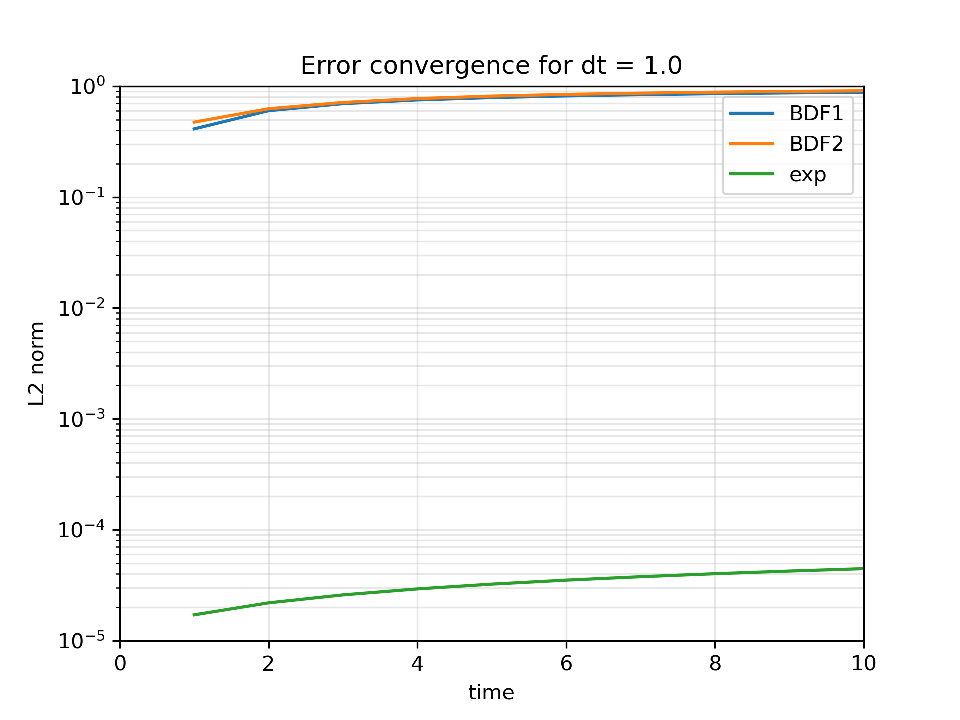
\includegraphics[width=0.5\linewidth]{res/homogeneo/L2norm_dt_1.0}
    &   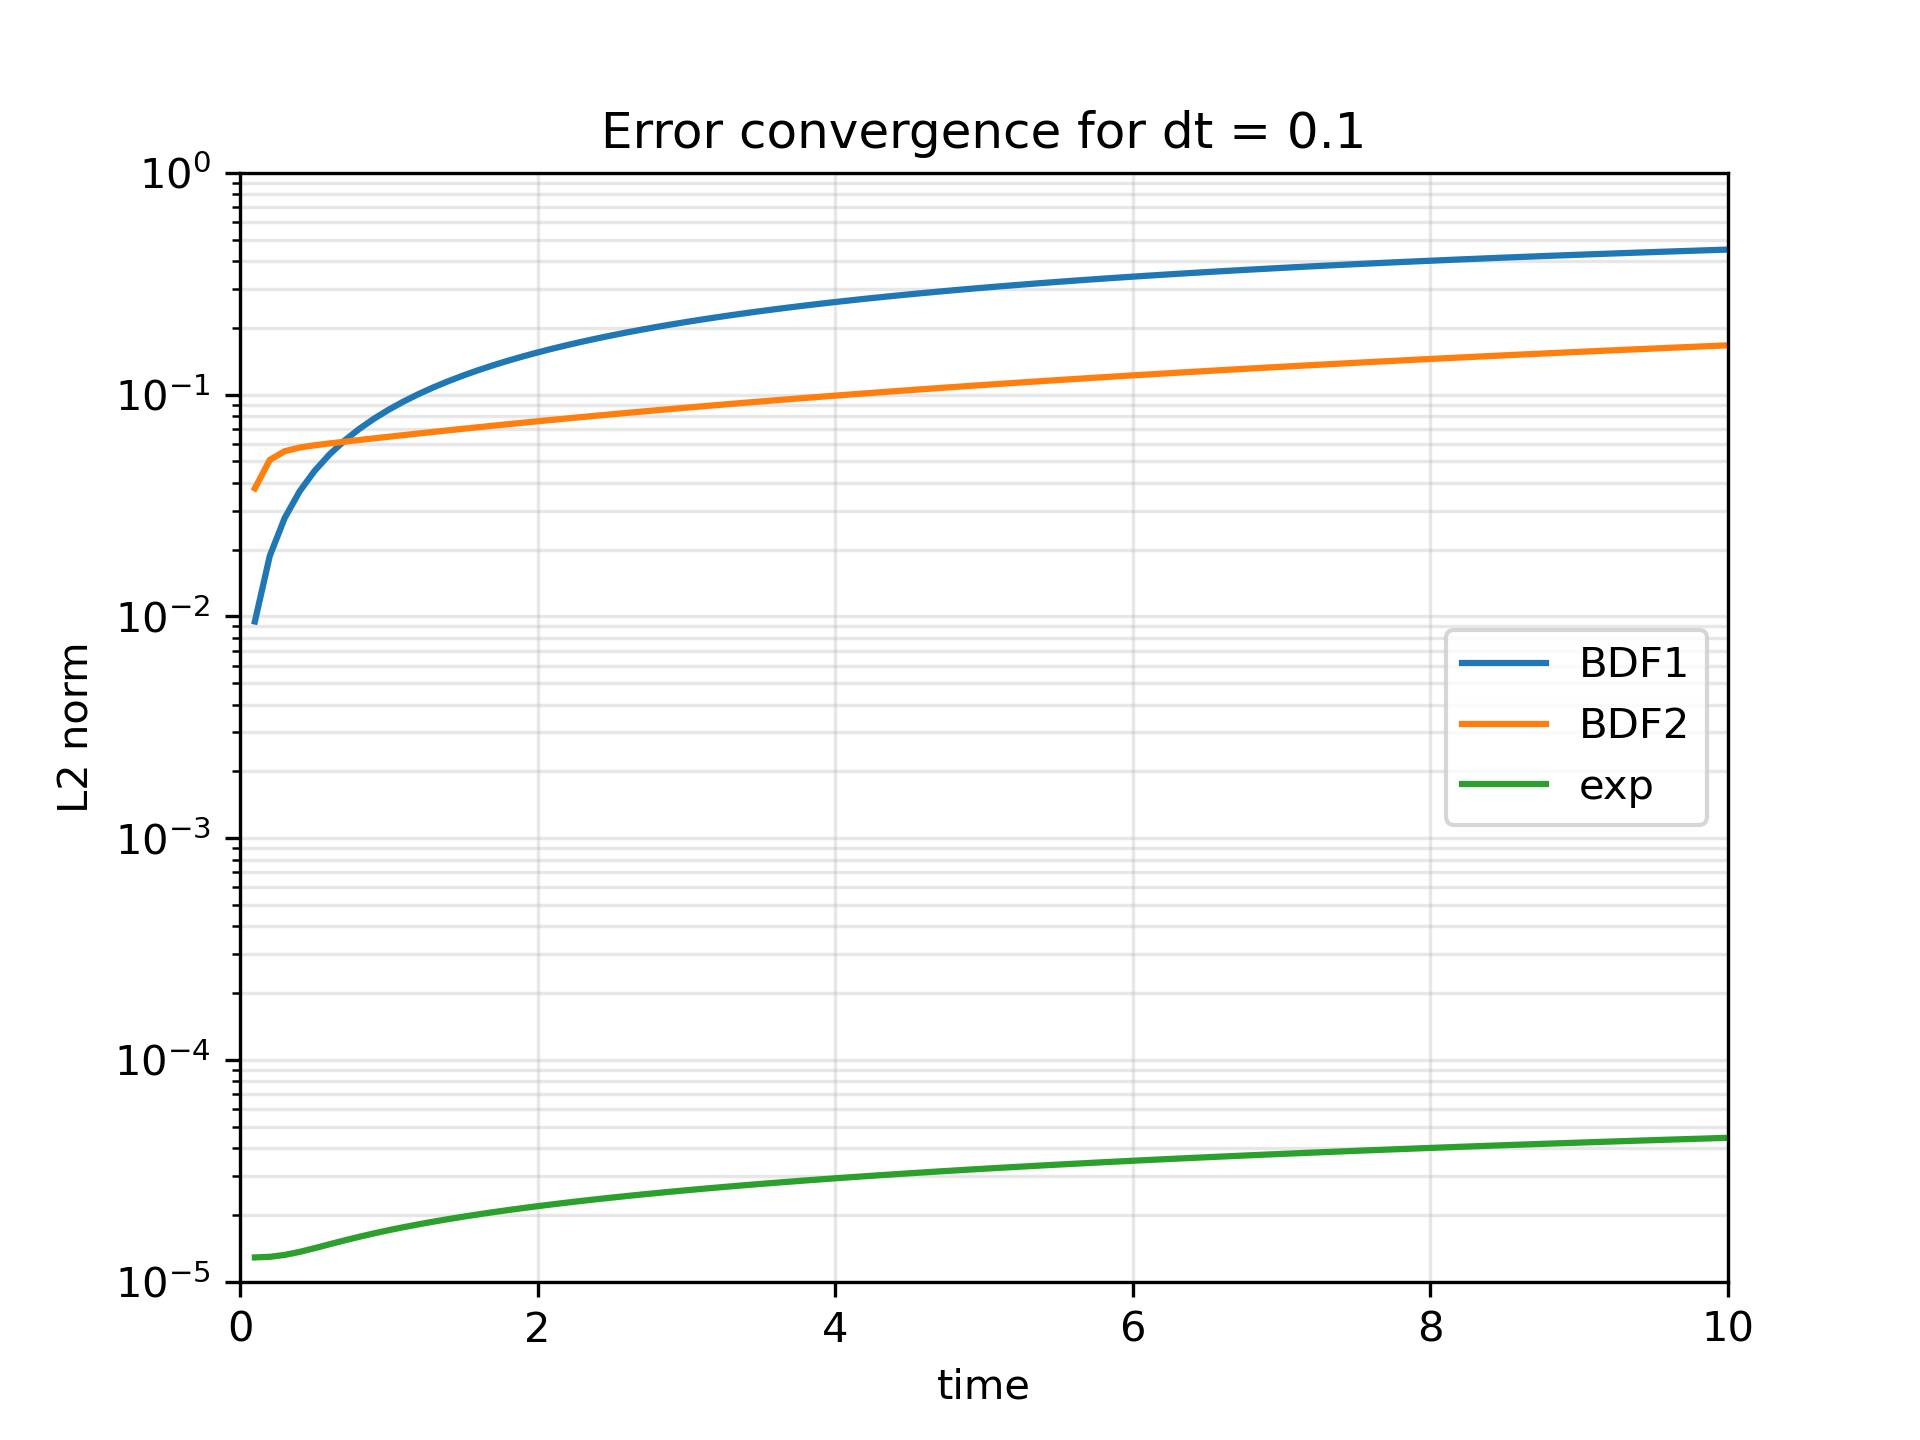
\includegraphics[width=0.5\linewidth]{res/homogeneo/L2norm_dt_0.1}
        \\
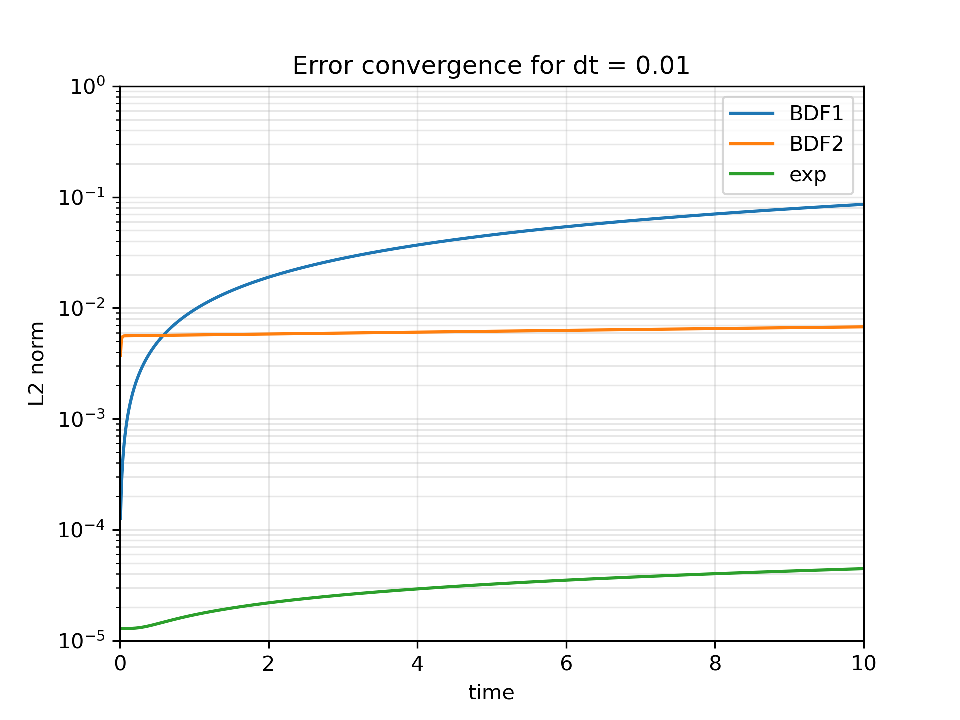
\includegraphics[width=0.5\linewidth]{res/homogeneo/L2norm_dt_0.01}
    &   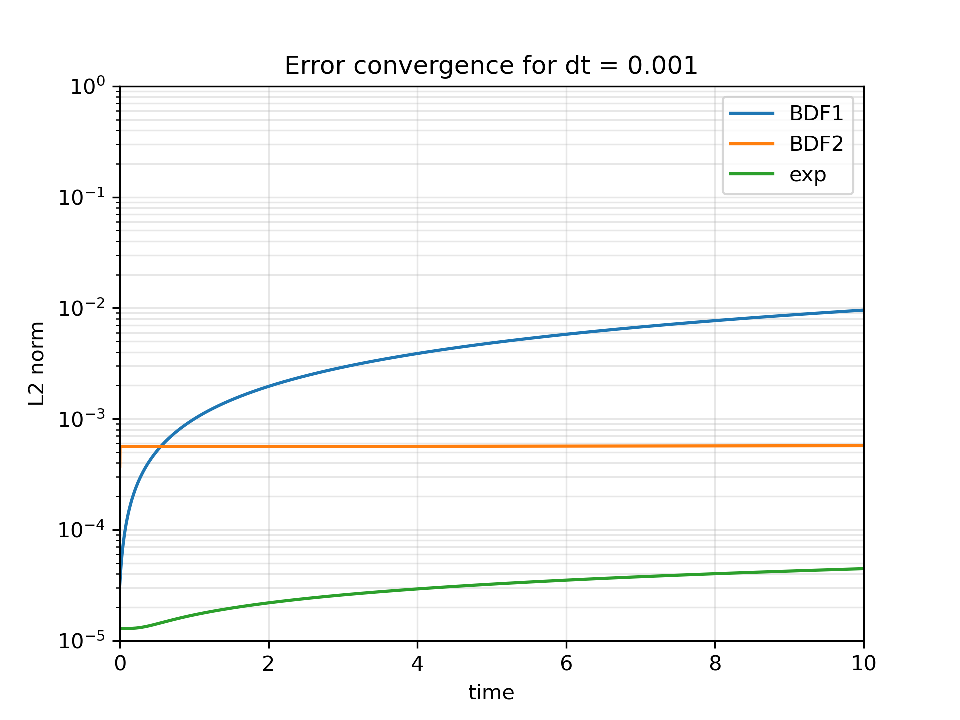
\includegraphics[width=0.5\linewidth]{res/homogeneo/L2norm_dt_0.001}
    \\
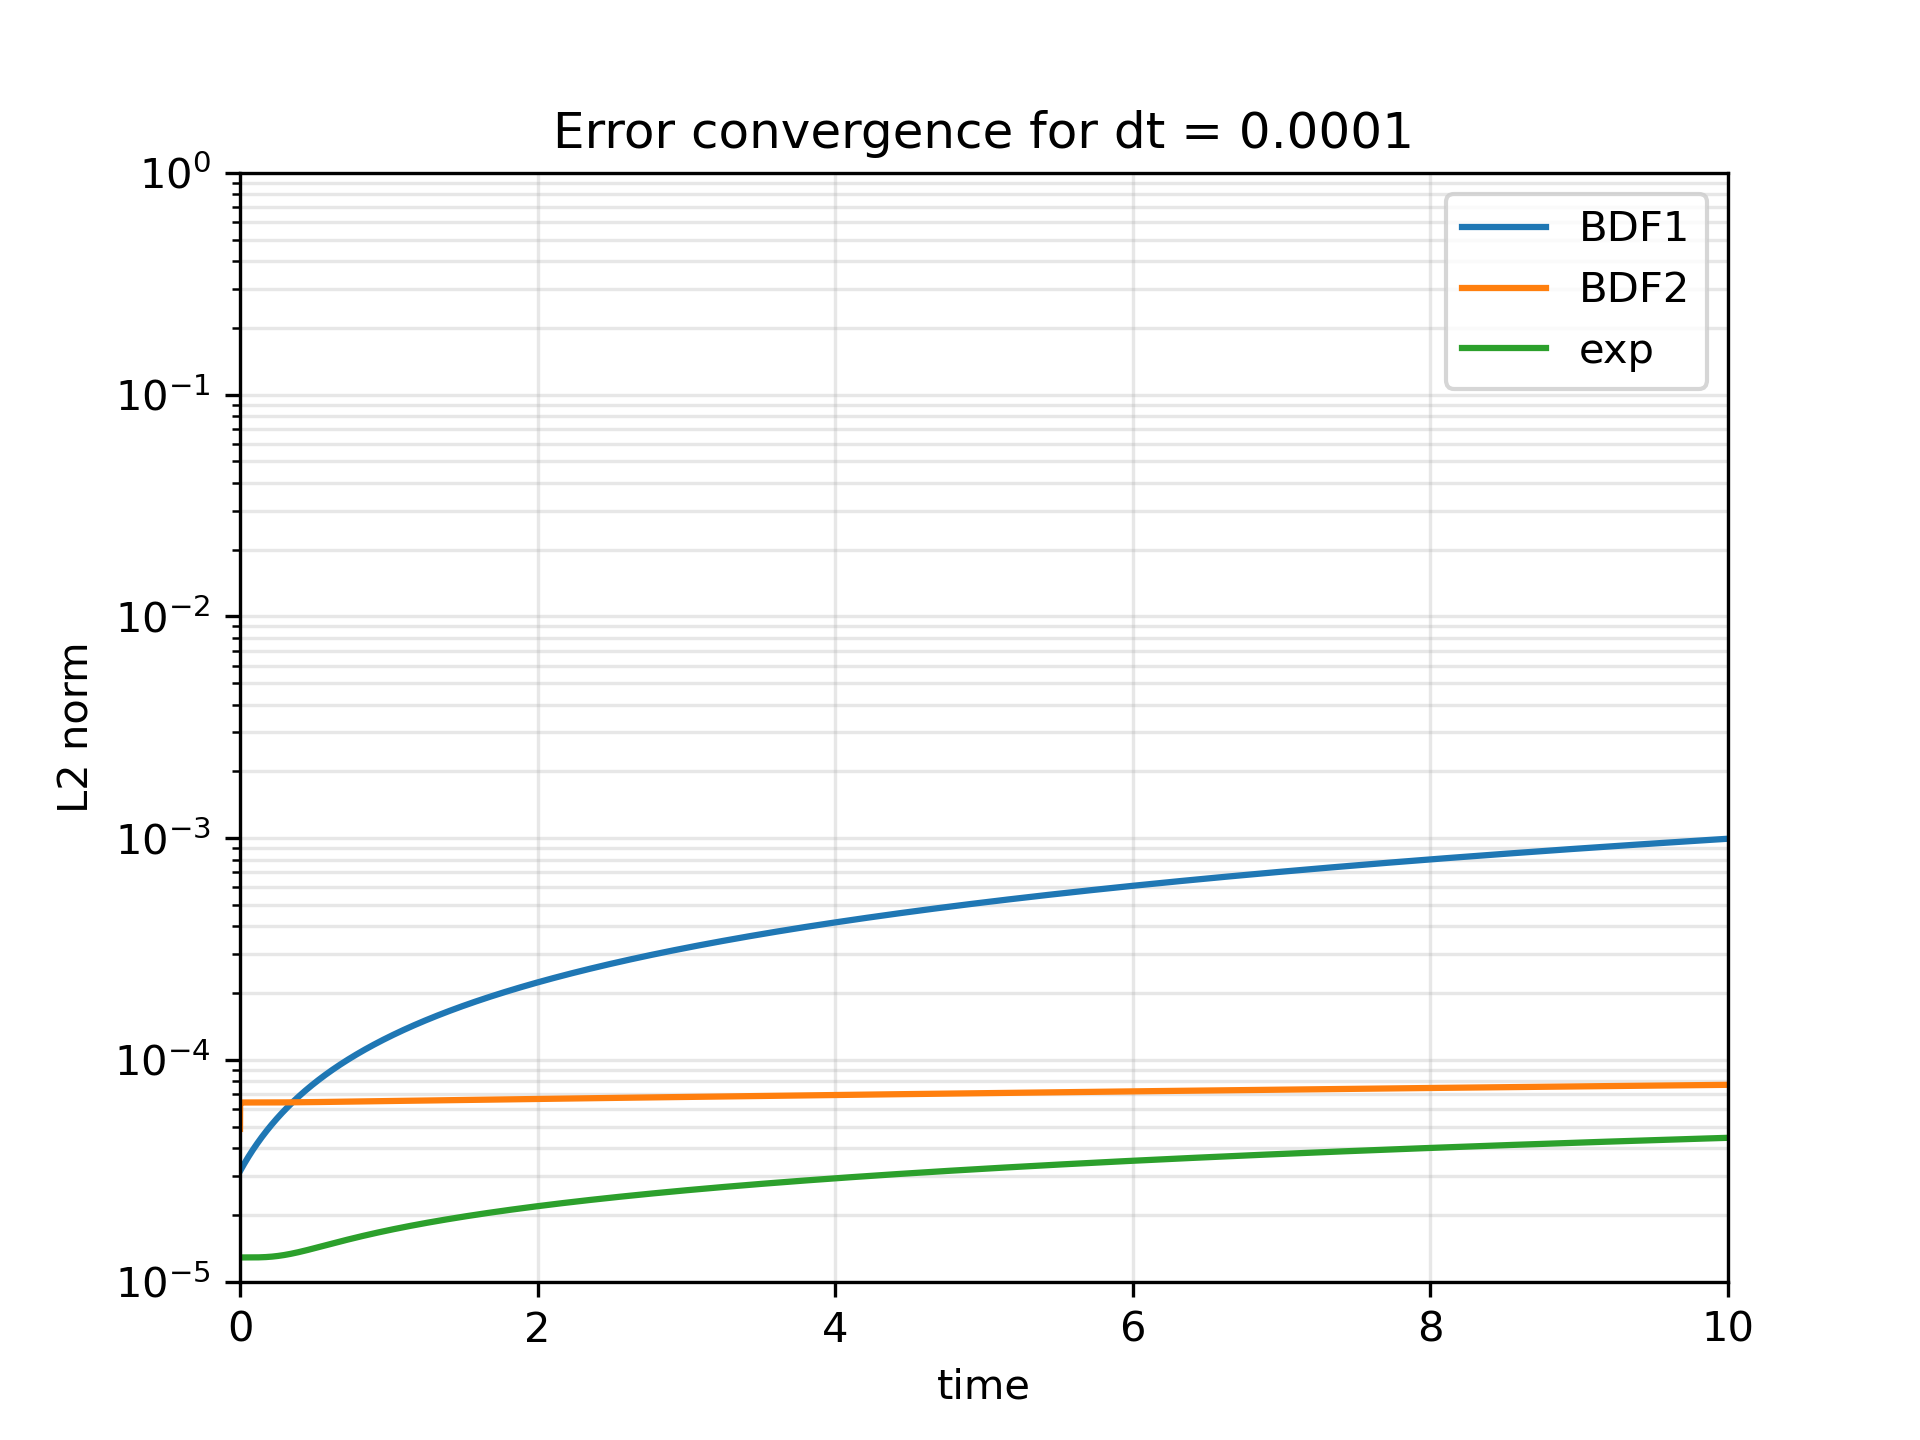
\includegraphics[width=0.5\linewidth]{res/homogeneo/L2norm_dt_0.0001}
&   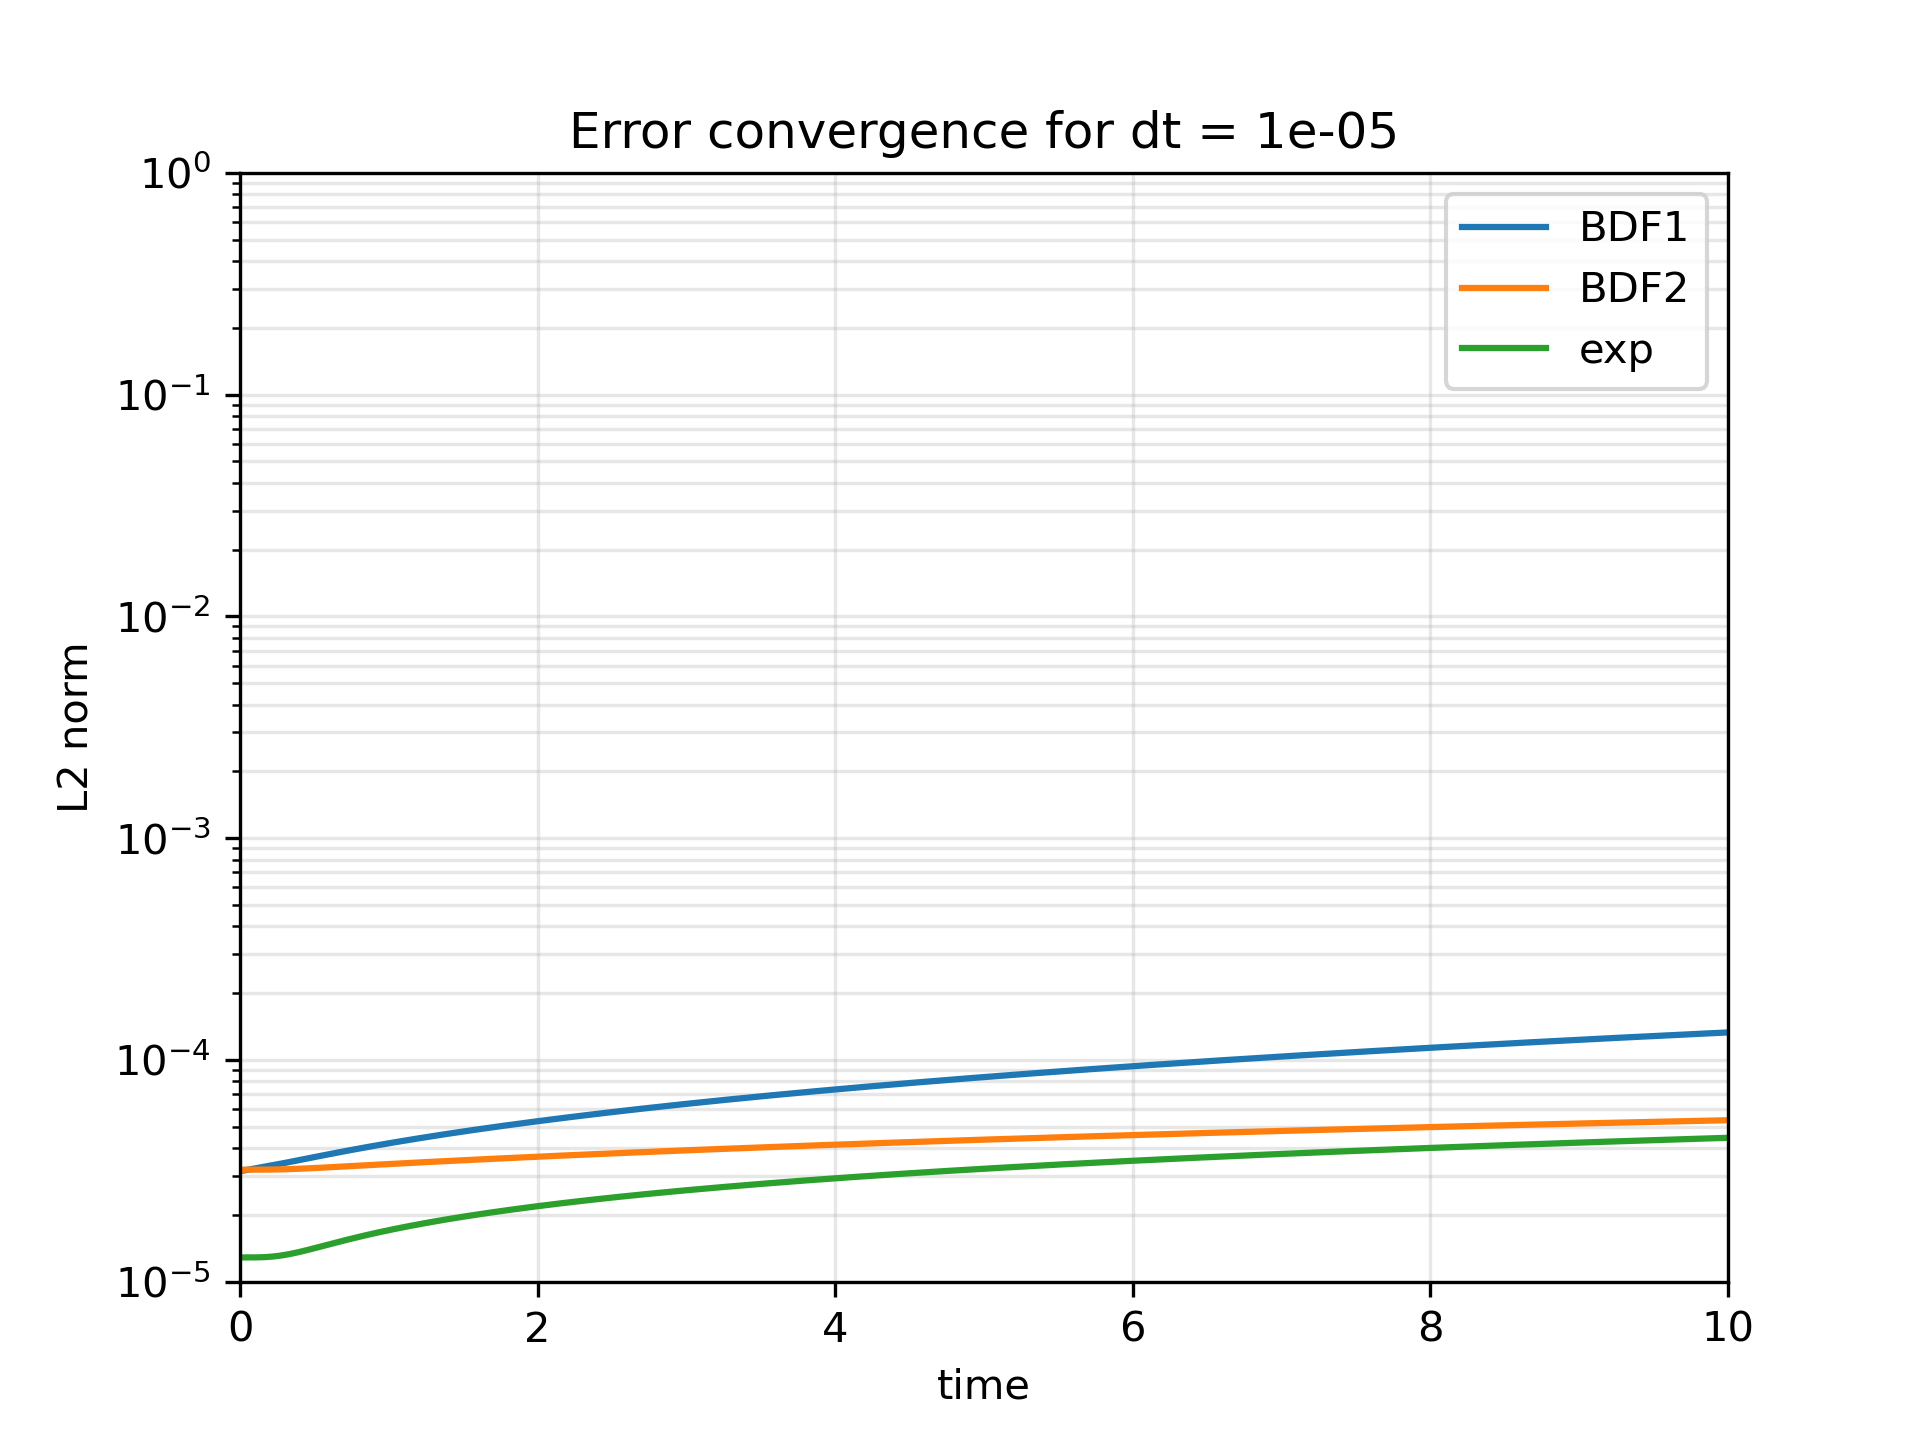
\includegraphics[width=0.5\linewidth]{res/homogeneo/L2norm_dt_1e-05}
     \end{tabular}
 
\caption{norma del error L2 en funci\'on del tiempo para  diferentes $\Delta t$}
\label{fig:conveg hom}
\end{figure}

En la figura (\ref{fig:conveg hom}) podemos observar la convergencia del error usando la norma L2  de el error $(u-u_h)$ , para $\Delta t = 0.01$ el esquema BDF3 presenta inestabilidades al punto de  diverge y oscilar cabe recordar aqu\'i que los m\'etodos  BDF De alto orden no son incondicionalmente estables \cite{Süli_Mayers_2003} como otros m\'etodos  expl\'icitos por lo que es de esperar este tipo de comportamientos al estar por fuera de la regi\'on de estabilidad. 


% idetificar cada delta de  t  el punto en la grafica  
\begin{figure}[H]
	\centering
	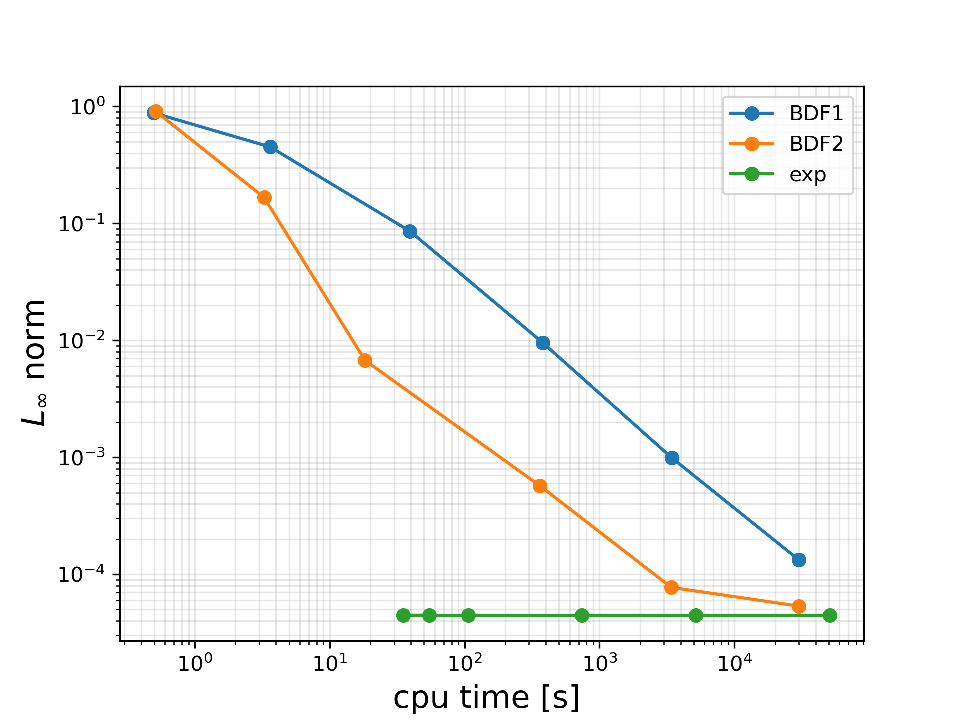
\includegraphics[width=0.7\linewidth]{res/homogeneo/cpu-L2.pdf}
	\caption{}
	\label{fig:tiempodecalculo H}
\end{figure}
% graficas : usando diferentes humbrales vs  cpu time 
En la figura (\ref{fig:tiempodecalculo H}) podemos ver las curvas del valor de la norma de error temporal $L_t$ \ref{t norm} en funci\'on del el tiempo de computo para cada uno de los esquemas temporales aqu\'i podemos demostrar la alta eficiencia de el m\'etodo de integraci\'on temporal a tal punto que para que los m\'etodos de mayor orden logren el mismo error los tiempos de computo para cada uno de los m\'etodos son equivalentes  si bien en deltas de tiempo pequeños la integracion exponencial requiere un tiempo de computo de casi un orden de magnitud mayor que otros esquemas dada la cantidad de bases necesarias para formar el sub espacio de krylov la ganancia en la precisi\'on  es indiscutible. 
 
\begin{figure}[H]
	\centering
	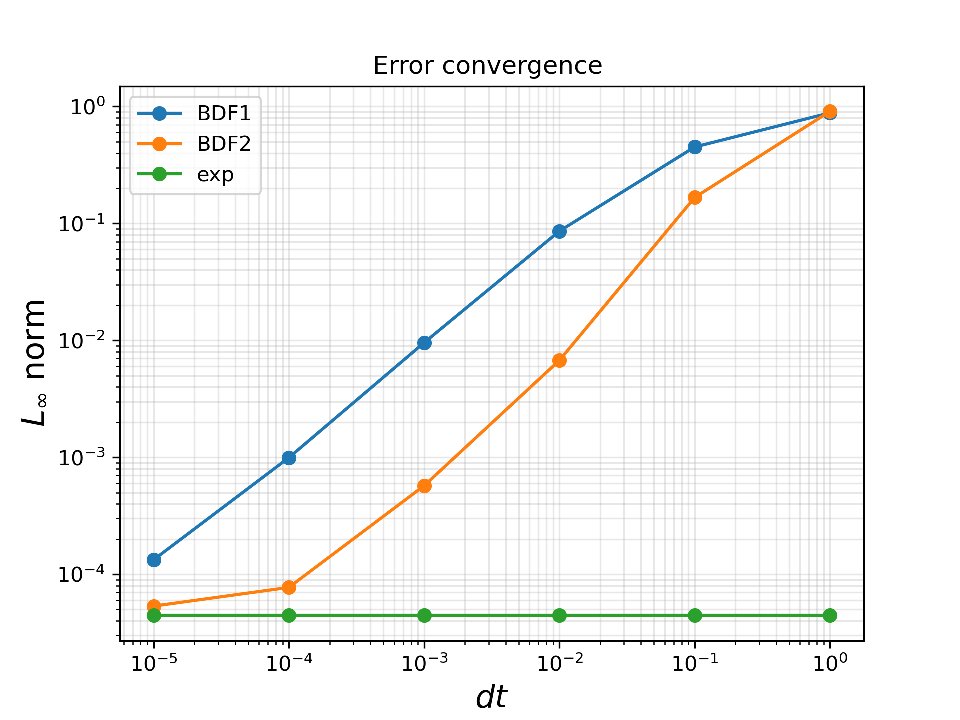
\includegraphics[width=0.7\linewidth]{res/homogeneo/dt-L2.pdf}
	\caption{}
	\label{fig:delta H}
\end{figure}

En la figura (\ref{fig:delta H}) podemos ver el compartimiento dependiente del delta de tiempo que poseen los esquemas BDF sin embargo el comportamiento de el metodo exponencial como se ha explicado anteriormente depende de la proyecci\'on en el subespacio de krylov mas que de el delta de tiempo con el que se avanza. 

\begin{figure}[H]
	\centering
	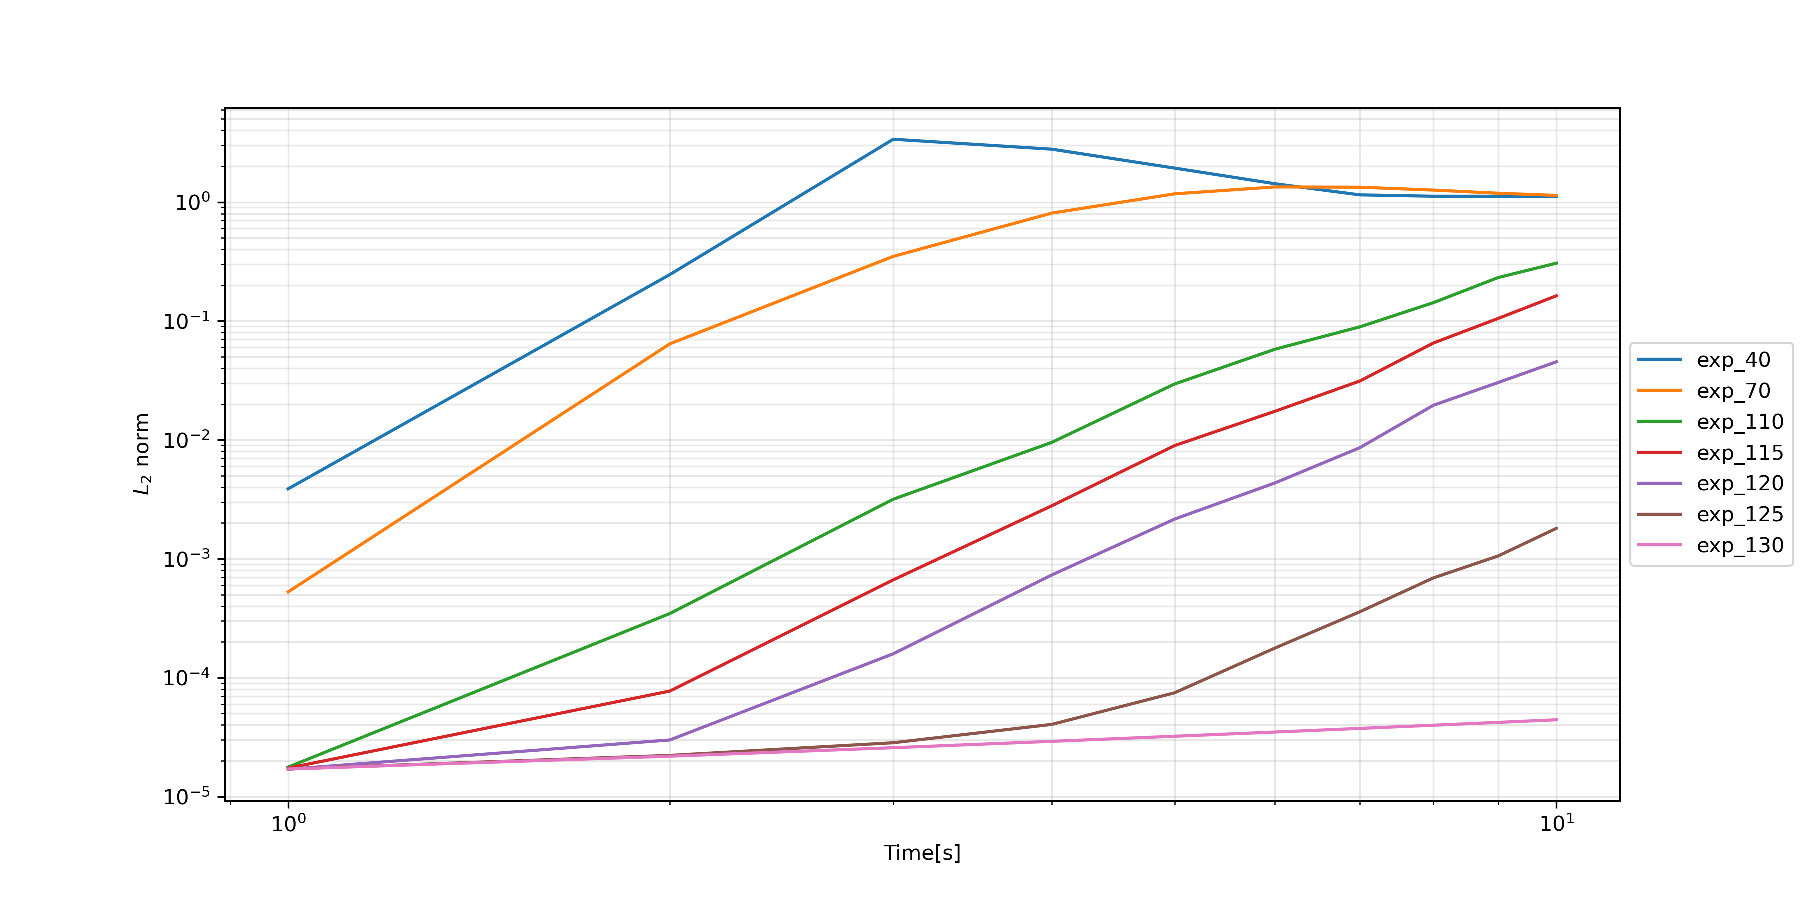
\includegraphics[width=0.7\linewidth]{res/homogeneo/L2norm_H_dim_dt_1.0.pdf}
	\caption{}
	\label{fig:H_dim h}
\end{figure}

\begin{figure}[H]
	\centering
	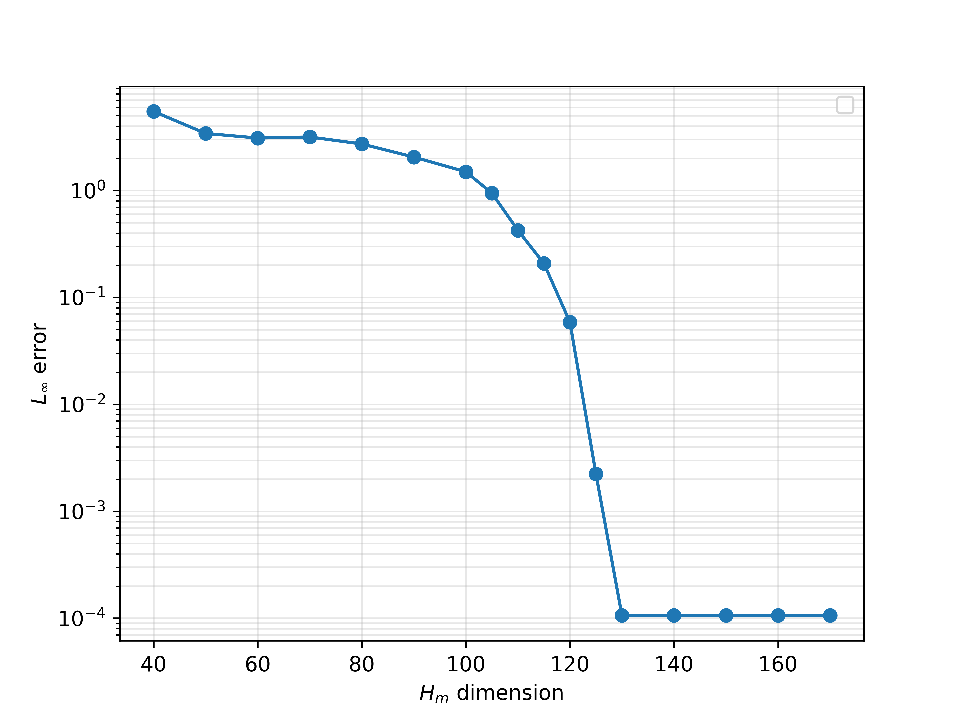
\includegraphics[width=0.7\linewidth]{res/homogeneo/H_dim.pdf}
	\caption{}
	\label{fig:dim h}
\end{figure}

En la figura (\ref{fig:H_dim h}) diferentes curvas de error para diferentes tamaños de proyecci\'on en el subespacio de krylov  y un m\'etodo de correcci\'on autom\'atico con una tolerancia de $1\times 10^{-14}$, aqu\'i podemos ver como es la fuerte dependencia de el error en conforme creamos un espacio de proyecci\'on mas grande para  a tal punto que como se ve en la figura(\ref{fig:dim h})  con fome se aproxima  el tamaño de la matriz 
Hessenberg a una dimensi\'on de sub espacio de krylov casi caracter\'istica el error cae r\'apidamente  cuando el tamaño de la proyecci\'on es mayor a  la dimensi\'on del sub espacio  las bases generadas con el algoritmo de arnoldi son en esencia vectores nulos la matriz de Hessenberg de rellena de ceros  y el error permanece constante    

\subsection{Problema No Homogeneo}

Para hallar un PDE no homog\'eneo con una soluci\'on anal\'itica conocida usaremos el m\'etodo de soluciones manufacturadas para proponer una soluci\'on y encontrar el termino fuente del problema al cual es soluci\'on \cite{Roache2019}, para esto tomaremos la soluci\'on al problema homog\'eneo (\ref{ana_ho}) podemos ver que $\lim_{t\to\infty} u(x,t)  = 0d$ si se añadimos un termino a esta soluci\'on sabremos que ese termino sera la soluci\'on estable del problema. \\

Teniendo esto en cuenta  podemos entonces proponer como soluci\'on la  funci\'on: 

\begin{equation}
    u(x,t) =\frac{1}{\sqrt{1+0.0004 t}}e^{- \frac{(x+t-3)^2}{0.0004t+1}} +x
    \label{ana_no_ho}
\end{equation}

Ahora hallamos el termino fuente de (\ref{Bench}) aplicando los operadores diferenciales. con lo que : 

\begin{equation}
    f = 1
\end{equation}

as\'i mismo sabemos que : 

\begin{equation}
    u(x,0) = \frac{1}{\sqrt{1+0.0004 t}}e^{- \frac{(x+t-3)^2}{0.0004t+1}} +x
\end{equation}


Sabemos que para este problema existe anal\'itica una soluci\'on del tipo:

\begin{equation}
    u(x,t) =\frac{1}{\sqrt{1+0.0004 t}}e^{- \frac{(x+t-3)^2}{0.0004t+1}}
\end{equation}

as\'i tambi\'en definiremos nuestras condiciones de contorno : 

\begin{align}
    u(0,t) &=  \frac{1}{\sqrt{1+0.0004 t}}e^{- \frac{(t-3)^2}{0.0004t+1}} \\
    u(20,t) &= \frac{1}{\sqrt{1+0.0004 t}}e^{- \frac{(17+t)^2}{0.0004t+1}}
\end{align}

\subsubsection{Resultados }
Para el an\'alisis del PDE no homog\'eneo se graficaron los mismo resultados que en el caso homogeneno figuras(\ref{fig:tiempodecalculo},\ref{fig:delta},\ref{fig:Hdim},\ref{fig:dim h}) presentando comportamientos en la precisi\'on de los m\'etodos id\'enticos 

\begin{figure}[H]
	\centering
	\begin{tabular}{cc}
		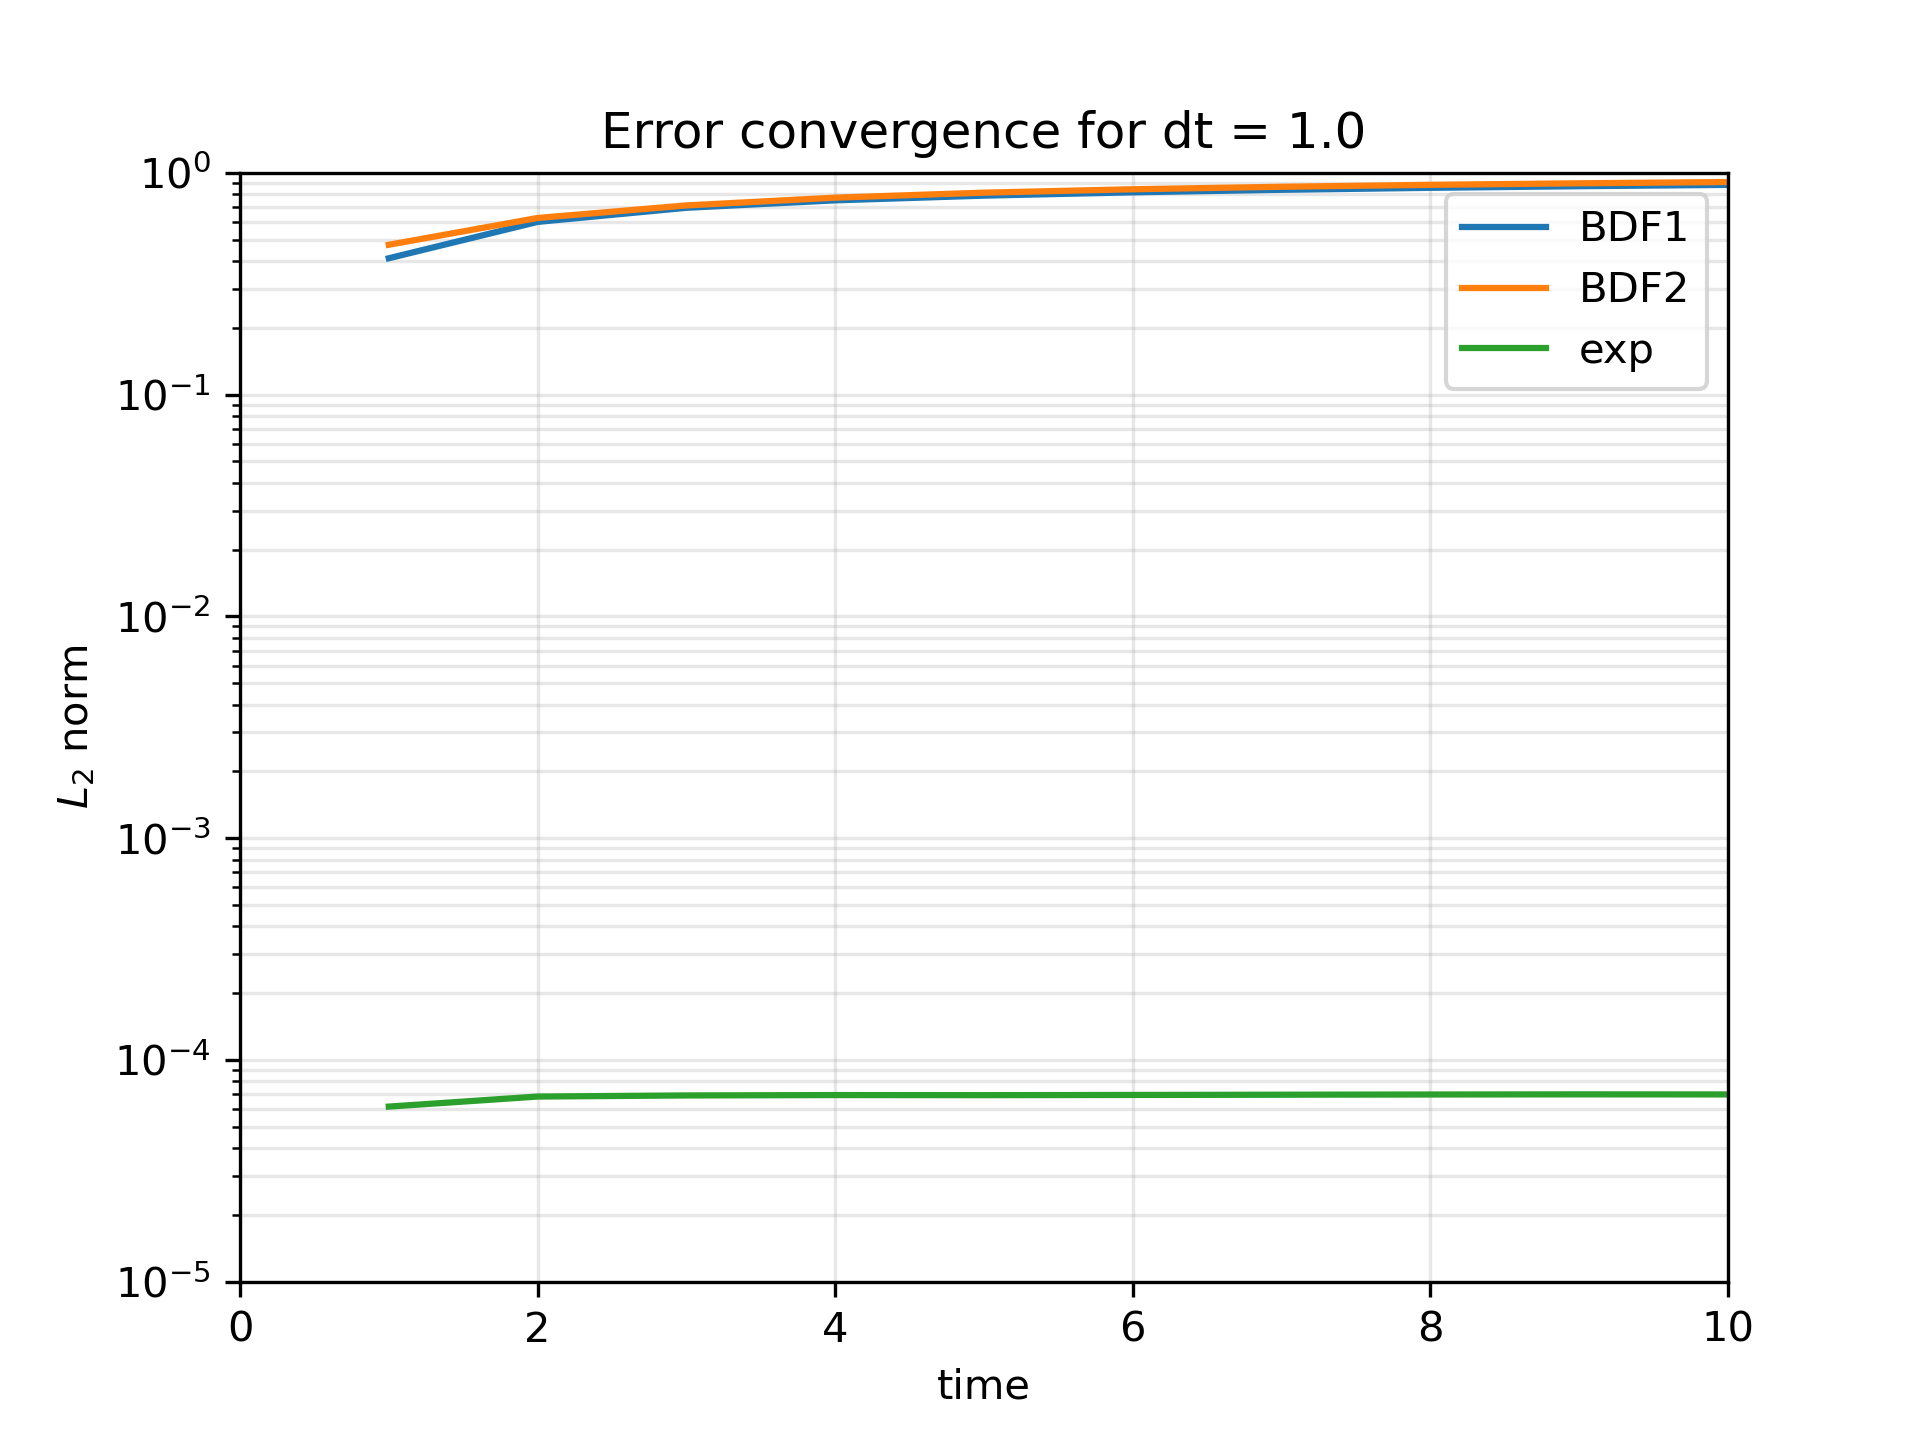
\includegraphics[width=0.5\linewidth]{res/no_homogeneo/L2norm_dt_1.0}
		&   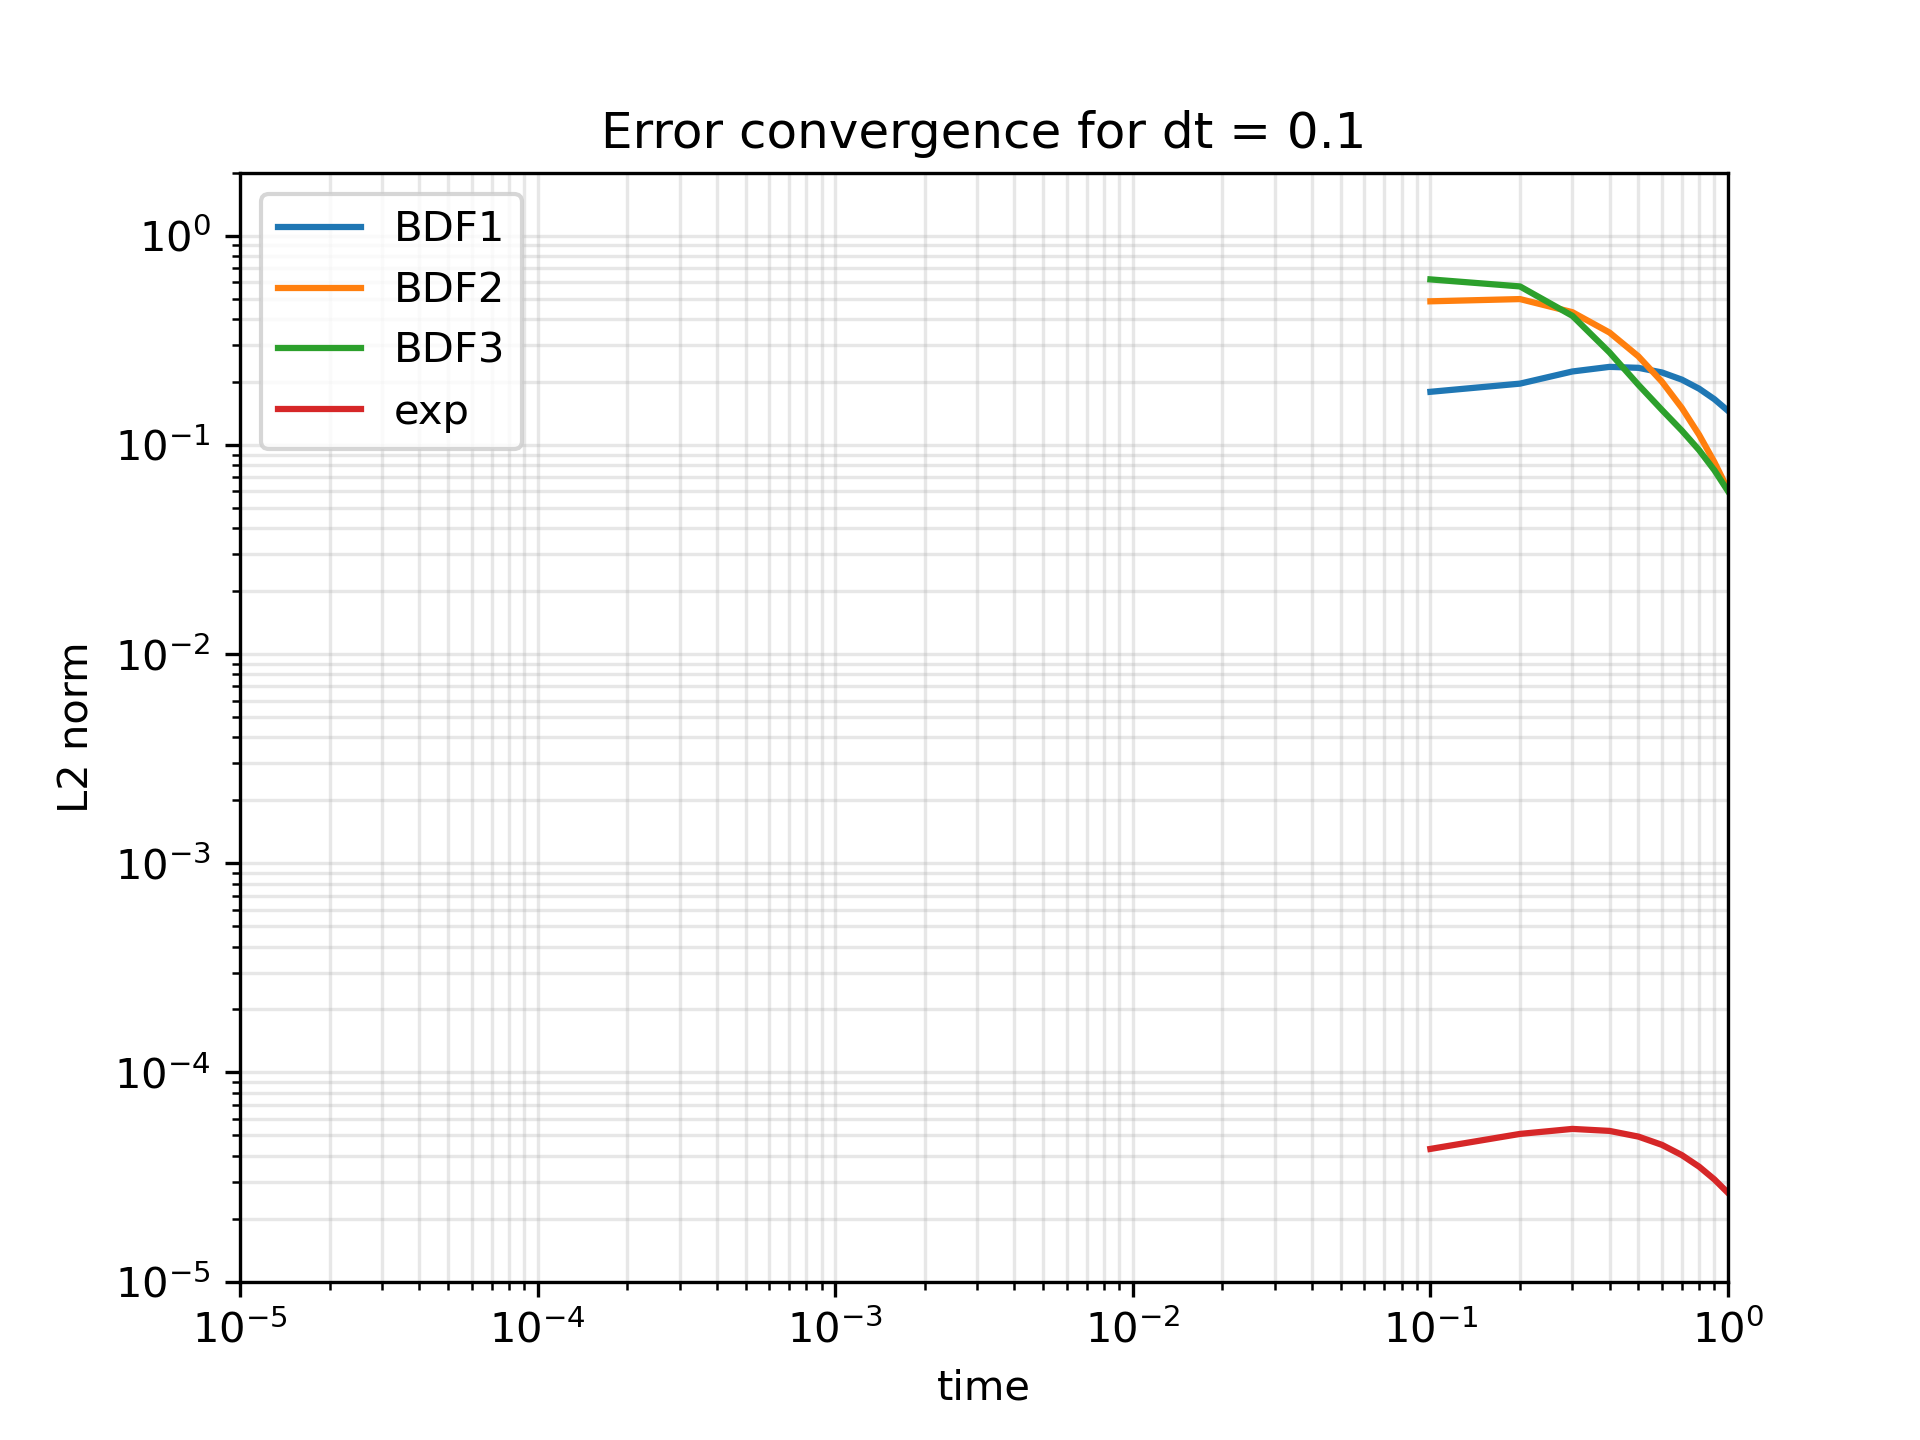
\includegraphics[width=0.5\linewidth]{res/no_homogeneo/L2norm_dt_0.1}
		\\
		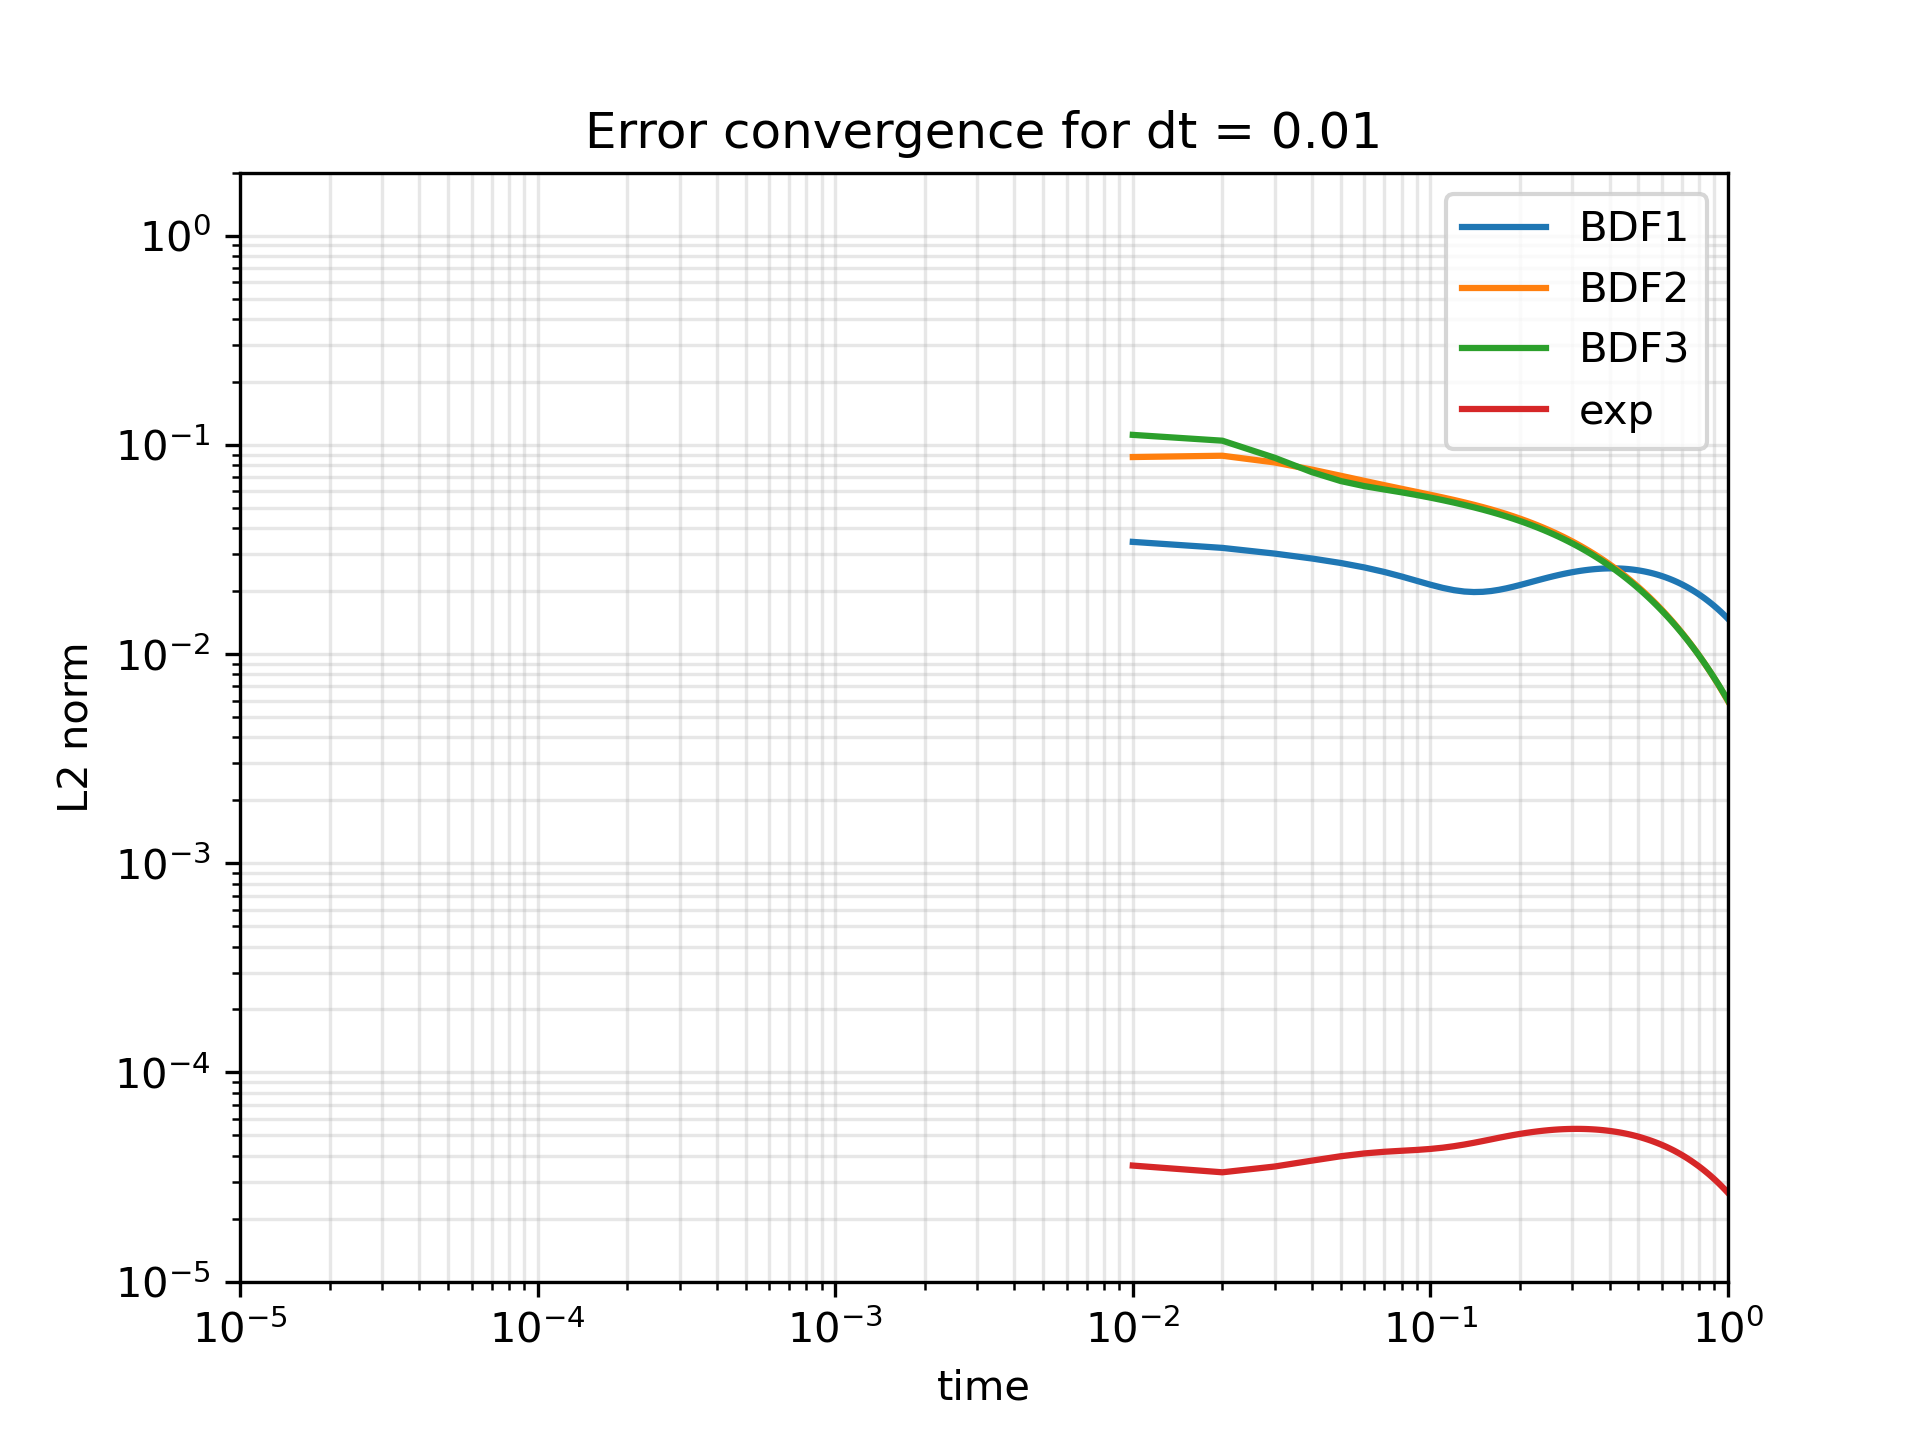
\includegraphics[width=0.5\linewidth]{res/no_homogeneo/L2norm_dt_0.01}
		&   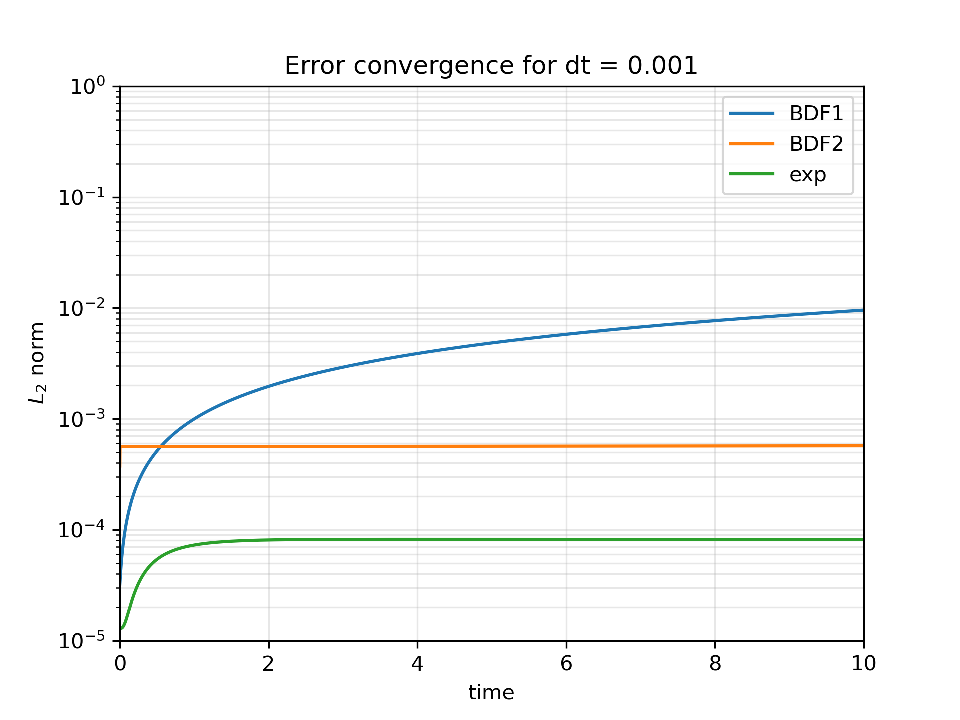
\includegraphics[width=0.5\linewidth]{res/no_homogeneo/L2norm_dt_0.001}
		\\
		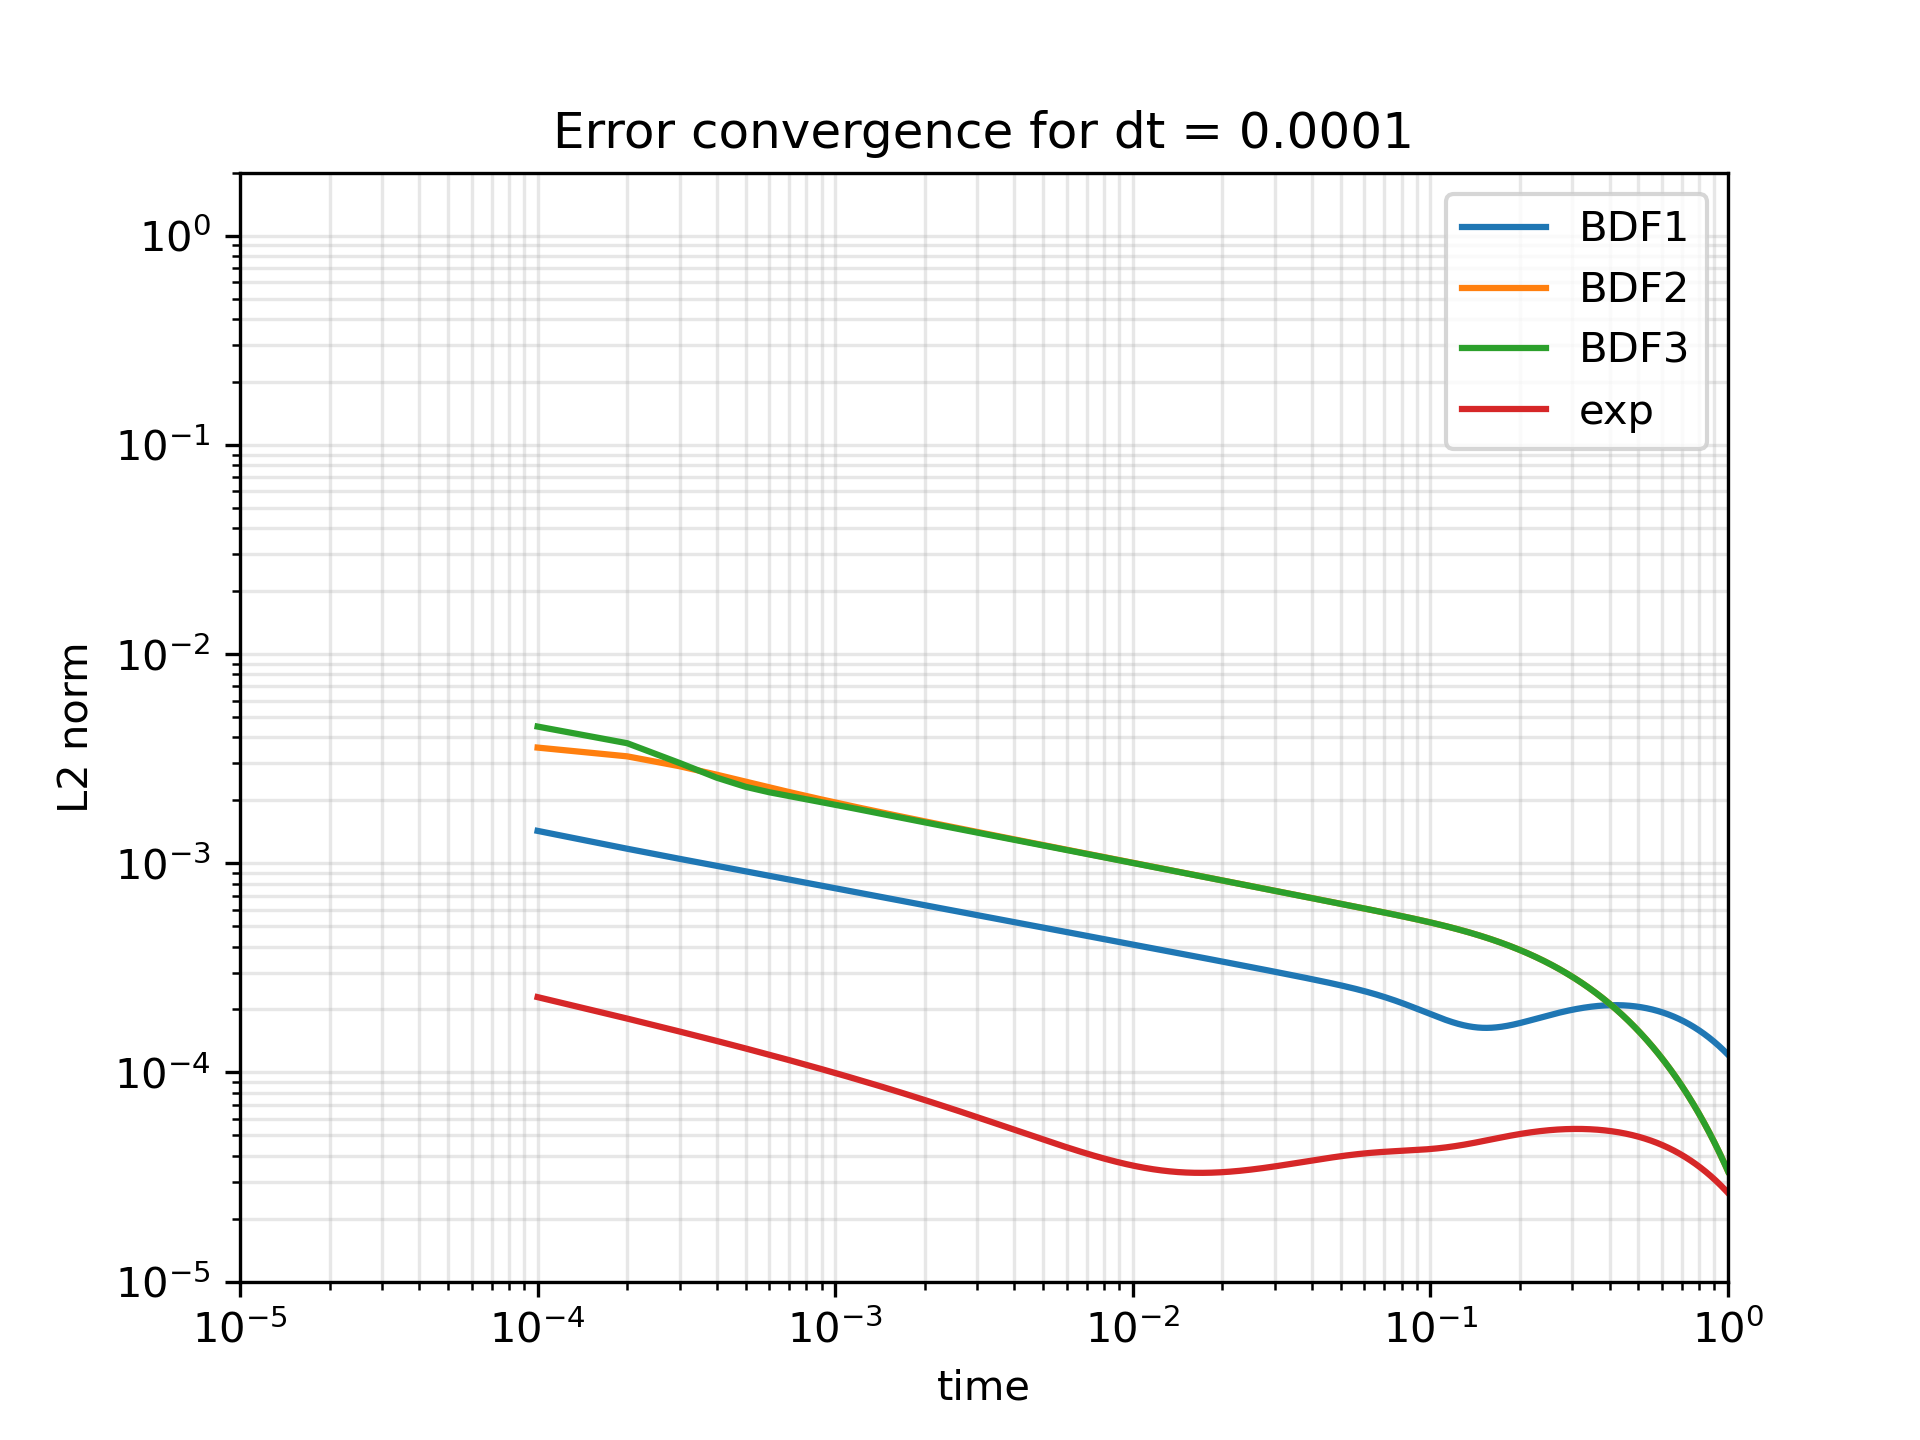
\includegraphics[width=0.5\linewidth]{res/no_homogeneo/L2norm_dt_0.0001}
		&   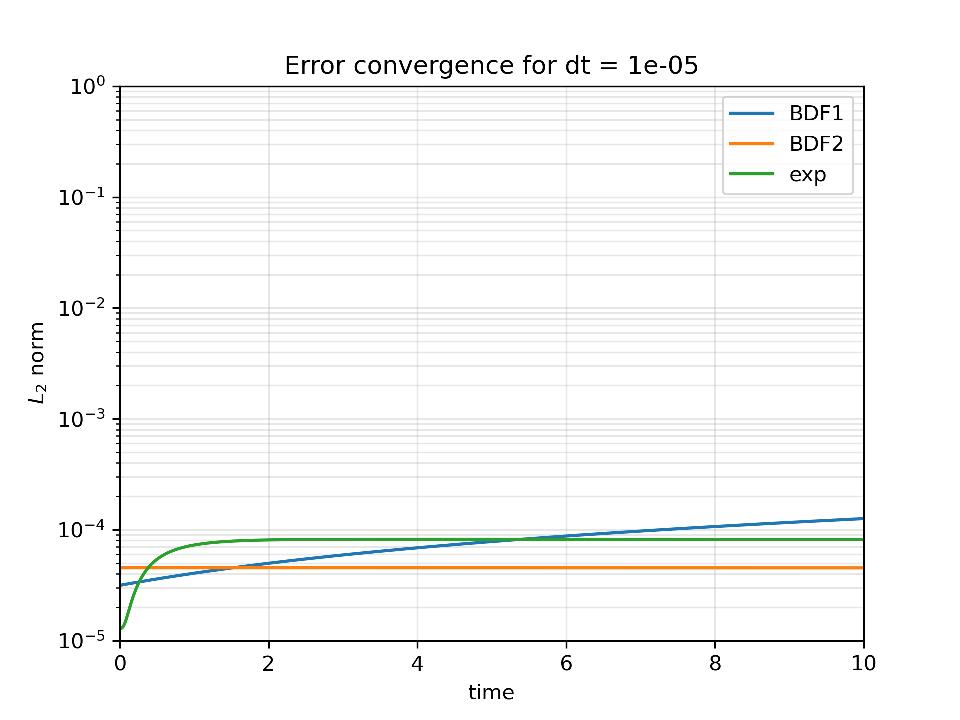
\includegraphics[width=0.5\linewidth]{res/no_homogeneo/L2norm_dt_1e-05}
	\end{tabular}
	
	\caption{norma del error L2 en funci\'on del tiempo para  diferentes $\Delta t$}
	\label{fig:conveg hom}
\end{figure}
En la figura (\ref{fig:convergence}) podemos observar la convergencia del error usando la norma L2  de el error $(u-u_h)$ , para el problema no homogenea presentamos el mismo inconveniente con la divergencia del esquema BDG3 al presentado en subproblema homogeneo.

\begin{figure}[H]
	\centering
	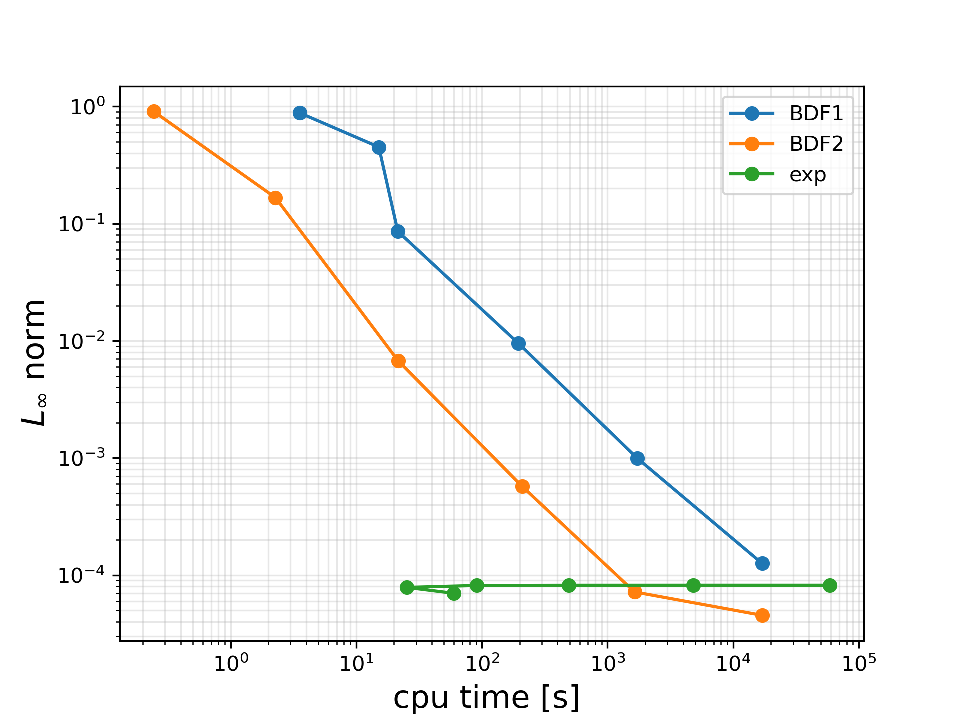
\includegraphics[width=0.7\linewidth]{res/no_homogeneo/cpu-L2.pdf}
	\caption{}
	\label{fig:tiempodecalculo}
\end{figure}

\begin{figure}[H]
	\centering
	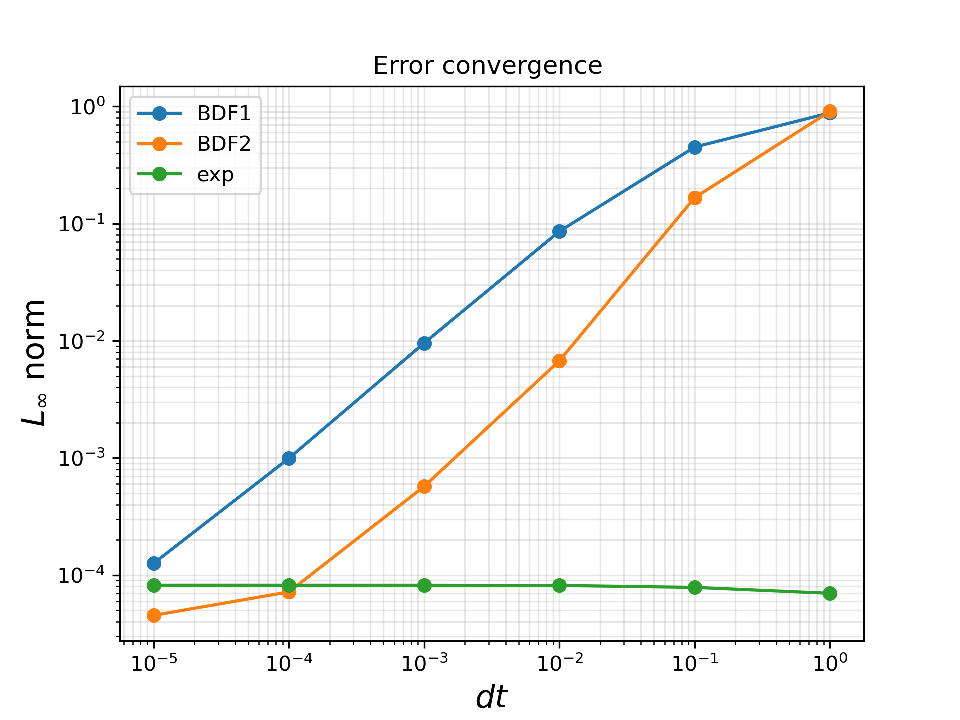
\includegraphics[width=0.7\linewidth]{res/no_homogeneo/dt-L2.pdf}
	\caption{}
	\label{fig:delta}
\end{figure}

\begin{figure}[H]
	\centering
	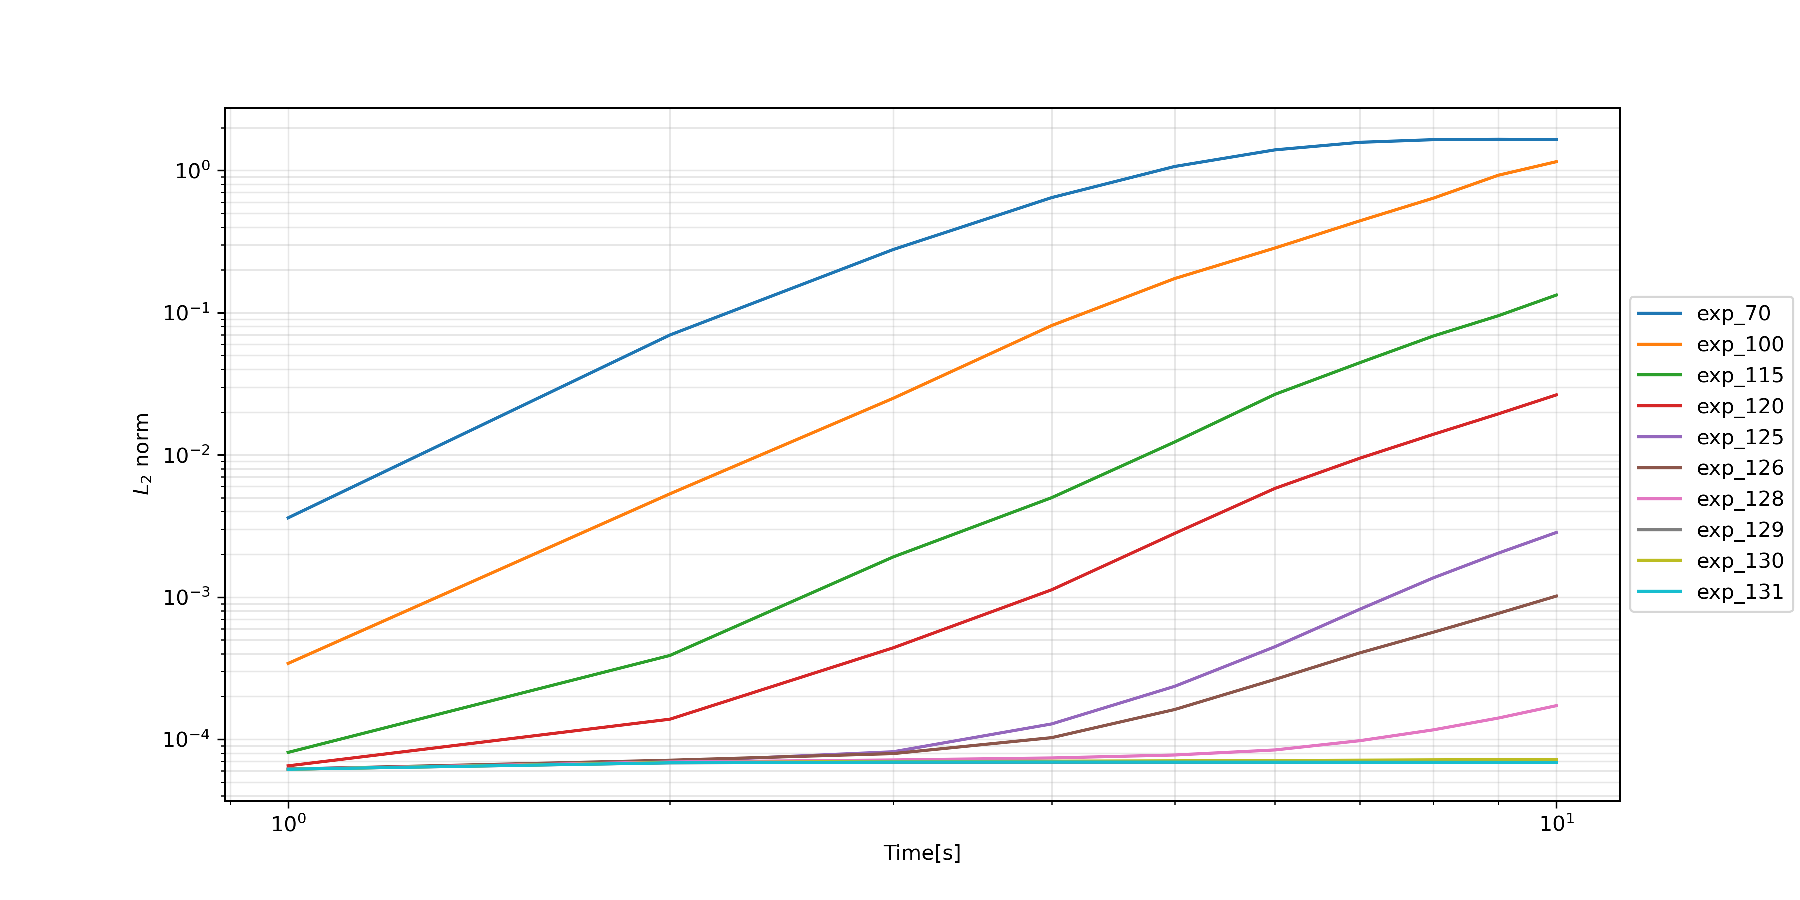
\includegraphics[width=0.7\linewidth]{res/no_homogeneo/L2norm_H_dim_dt_1.0.pdf}
	\caption{}
	\label{fig:Hdim}
\end{figure}

\begin{figure}[H]
	\centering
	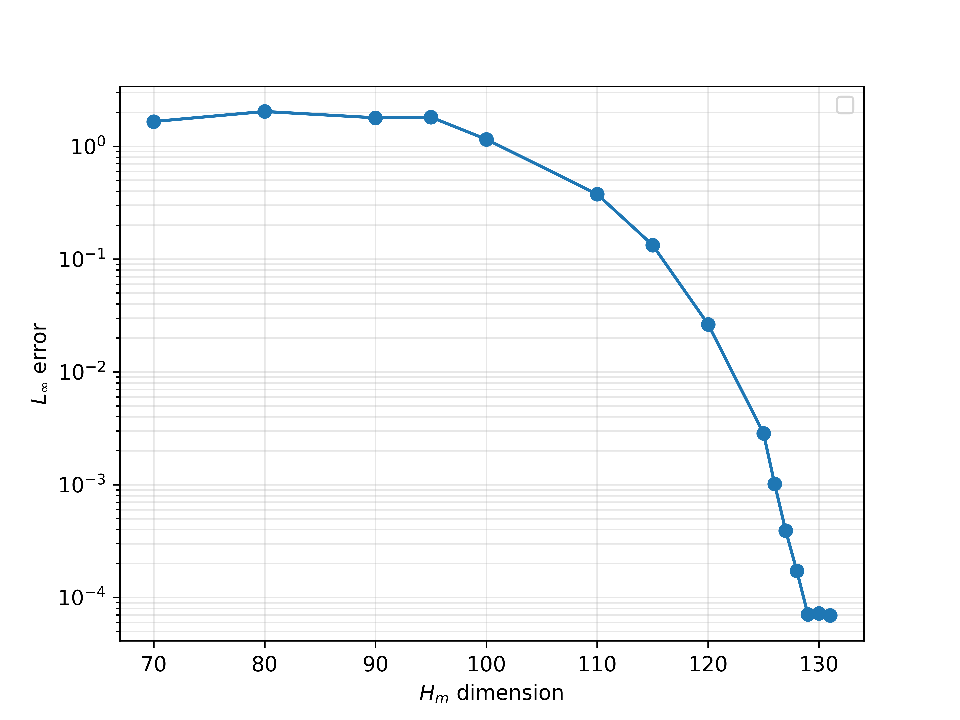
\includegraphics[width=0.7\linewidth]{res/no_homogeneo/H_dim.pdf}
	\caption{}
	\label{fig:dim h}
\end{figure}



\section{Conclusiones}
De el estudio realizado podemos concluir que el m\'etodo de integraci\'on exponencial es una ventaja en los problemas convectivos difusivos ya que su precisi\'on no depender\'a de el termino $\delta t$.

Una caracter\'istica de la no dependencia de el $\Delta t$ que tomemos es en cambio el costo computacional dado que el tamaño del sub espacio de krylov de tamaño $m$ y que el criterio de error para esta proyecci\'on requiere evaluar el exponencial de la matriz de Hessenberg resultante por lo que al requerir de un mayor numero de bases los tiempos de c\'omputos con significativos pero incluso aun inferiores a los necesarios para lograr el mismo tamaño de error . 

Usar un \'unico tamaño de proyecci\'on para la matriz de Hessenberg resulta si bien mas econ\'omico computacional es dif\'icil asegurar un bajo error dado que no se conoce la dimensi\'on del sub espacio de krylov para esa matrix vector $A$ , $v$ dado que v varia en el tiempo sera la misma en todos los instantes y se tendria que asegurar que el tamaño $ l $ elegido cumpla 


\printbibliography

\end{document}
